\RequirePackage{amsmath}
\documentclass[a4paper]{article}
\usepackage[T1]{fontenc}
\usepackage[french]{babel}
\usepackage[utf8]{inputenc}

\usepackage[dvipsnames]{xcolor}
\usepackage{changepage}
\usepackage{xr}
\usepackage{float}
\usepackage{array}
\usepackage{booktabs}
\usepackage{graphicx}
\usepackage{pdfpages}
\usepackage{tabularx}
\usepackage{multirow}
%\usepackage{fancyhdr}
%\pagestyle{fancy}
%\fancyhead{}
%\fancyhead[RO,LE]{CHAPTER \thechapter}
\setlength{\headheight}{15pt} 
\usepackage{hyperref}
\hypersetup{
    colorlinks,
    citecolor=OliveGreen,
    %filecolor=black,
    linkcolor=OliveGreen,
    urlcolor=black
}
\usepackage{minitoc}
\usepackage{silence}
\WarningFilter{minitoc(hints)}{W0028} %chktex-file 36
\WarningFilter{minitoc(hints)}{W0024}
\WarningFilter{minitoc(hints)}{W0023}
\WarningFilter{minitoc(hints)}{W0030}
\WarningFilter{minitoc(hints)}{W0039}
\graphicspath{{./img/}}
\usepackage[toc,page,title]{appendix}
\usepackage[caption=false]{subfig}
\usepackage[titlenumbered, ruled]{algorithm2e}
\SetKwRepeat{Do}{do}{while}
\DeclareGraphicsExtensions{.pdf,.png,.jpeg,.jpg}

\begin{document}

\title{Contributions aux communications inter-vues pour l'apprentissage collaboratif\\~\\
\large Résumé de thèse}
\author{Denis Maurel}
\date{}

\maketitle

\section{Contexte}
Cette thèse portant sur l'étude des communications au sein de modèles d'apprentisage automatique collaboratif a été dirigée par Raja Chiky (ISEP) et co-encadrée par Jérémie Sublime (ISEP) et Sylvain Lefebvre (ISEP).\\

L'objectif principal de cette thèse était d'étudier les communications inter-vues au sein de modèles d'apprentissage collaboratifs afin d'améliorer la transmission d'informations entre les vues. Cette idée a été déclinée suivant deux axes en fonction du type d'application concerné:\\

\begin{itemize}
    \item Le clustering collaboratif pour lequel chaque vue disposera initialement d'un clustering local qui sera ensuite modifié afin d'arriver à une série de concensus entre les vues. La modification de chaque clustering local se base sur l'échange d'informations entre les vues, afin que les resultats obtenus localement puissent être utilisés par les vues externes. Le clustering collaboratif s'attache à trouver un concensus aussi global que possible plutôt qu'à améliorer chaque clustering local. Le clustering collaboratif est à distinguer de l'Ensemble Learning qui lui cherche à trouver un concensus unique entre toutes les vues à l'aide d'une fusion au sein d'un modèle global de l'ensemble des clusterings locaux. Au sein de cette thèse, nous parlerons majoritairement de la version horizontale du clustering collaboratif, pour laquelle chaque vue dispose du même ensemble d'individus décrits au sein de chaque vue par un ensemble différent de caractéristiques. Deux sous-axes ont été explorés concernant les communications inter-vues:
        \begin{enumerate}
            \item L'optimisation des coefficients définissant l'importance que chaque vue accorde à l'information reçue de ses paires. Pour cela nous proposons une nouvelle méthode d'apprentissage permettant d'adapter dynamiquement ces poids à l'aide d'un apprentissage.
            \item La proposition d'une méthode d'apprentissage au cours du temps (que nous qualifierons d'en ligne) permettant à des vues de communiquer au fil du temps afin de faire évoluer les résultats obtenus localement à d'éventuels changements de distribution.
        \end{enumerate}

    \item La reconstruction collaborative dont le but est de reconstruire localement des données manquantes à l'aide d'informations présentes dans les vues externes. Cette application est développée dans cette thèse avec la proposition d'un système permettant d'inférer l'approximation d'un individu à l'aide entre autre de réseaux de neurones. Ces réseaux seront utilisés soit pour coder l'information à transférer afin d'assurer une sécurité minimum, soit pour inférer les valeurs locales d'un individu en se basant sur l'information reçue de la vue externe.
\end{itemize}


\section{Clustering collaboratif}


Le clustering collaboratif est défini par un ensemble de base de données (appelées vues) ayant chacune opéré un clustering sur leurs données locales. Le but du clustering collaboratif va être de faire s'échanger de l'information entre les vues afin de modifier chaque clustering local pour finalement se rapprocher d'un concensus entre les vues.\\

Se pose alors le problème du recoupement d'information lorsqu'une vue locale reçoit des informations provenant de plus d'une source externe. Les méthodes existantes dans l'état de l'art se basent sur une pondération de ces informations à l'aide de coefficients scalaires~\cite{cornuejols2018collaborative,pedrycz2002collaborative,maurel2017incremental,ghassany2012collaborative,sublime2016collaborative,rastin2015collaborative}. Cependant, la méthode de définition de ces coefficients est à chaque fois empirique, et c'est sur ce constat que se basent les travaux présentés dans la première partie de cette thèse. Un second constat après étude de l'état de l'art a été qu'il n'existait actuellement pas de méthode permettant d'effectuer un apprentissage en ligne (au cours du temps) de modèles collaboratifs. Un second sous axe d'exploration a ainsi consisté en la modification d'une méthode existante de clustering collaboratif~\cite{ghassany2012collaborative} basée sur des cartes auto adaptatrices~\cite{KOHO1} afin de l'adapter à l'apprentissage en ligne. Ces travaux étaient de plus motivés par la volonté de rendre les modèles collaboratifs réactifs aux éventuels changement au cours du temps dans la distribution des données.

L'ensemble des travaux présentés dans cette section se base sur la fonction de co\^{u}t définissant le score du modèle à chaque instant:

\begin{align}
    \label{eq:sum_globalC}
    Q^i &= \alpha_i Q^i_{local}(V_i) + Q^i_{collab}(V_i, V_{j\neq i})\\
    &= \alpha_i Q^i_{local}(V_i) + \sum_{j\neq i} \beta_i^j C_j^i(V_i, V_j)
\end{align}

Ces formules contiennent l'ensemble des éléments nécessaires pour définir un problème de clustering collaboratif. $Q$ représente à chaque fois un critère d'évaluation, $Q^i$ représente la valeur de ce critère pour la $i$-ème vue $V_i$, avec une distinction entre $Q^i_{local}$ et $Q^i_{collab}$ qui définissent les critères sur respectivement les résultats locaux du clustering ainsi que sur l'état du concensus entre les vues. $C_j^i$ définit la dissimilarité entre les vues $V_i$ et $V_j$. La pondération entre le critère local et les différentes mesures de similiraités est assurée par l'ensemble de coefficients $\alpha_i$ et $\beta^j_i$ donc la fonction et la définition sont donnés dans la section suivante.

À noter que les définitions des critères $Q_{local}$ et $Q_{collab}$ sont propres soit à l'algorithme de clustering local utilisé dans chaque vue~\cite{ghassany2012collaborative}, soit à la définition même du problème de clustering~\cite{sublime2018information}. Dans les deux cas, le critère doit être redéfini pour chaque problème.

\subsection{Optimisation des poids pour du clustering collaboratif basé sur des cartes auto adaptatrices}

Nos contributions presentées dans cette section sont les suivantes:
\begin{itemize}
    \item Nous proposons une méthode d'optimisation automatisée et non-supervisée afin d'ajuster la valeur des coefficients définissant l'importance que les vues doivent mutuellement s'accorder lors de leur apprentissage collaboratif.
    \item Nous démontrons expérimentalement que notre méthode d'optimisation est capable de détecter les vues bruitées qui auraient pu détériorer les apprentissages finaux.
    \item Nous fournissons les propriétés théoriques de notre méthode. En particulier, nous montrons que notre méthode d'optimisation définit un méta-clustering sur les vues, en les regroupant suivant leurs similarités.
\end{itemize}

La définition de notre méthode d'optimisation s'est faite grâce à l'ajout de deux contraintes au problème initial. La première a été que, quelque soit la vue $V_i$, la valeur associée à $Q^i_{local}$ devrait être égale à $\alpha_i=1$. Cette contrainte traduit le fait qu'en divisant l'ensemble des $\beta^j_i$ par $\alpha_i$ dans l'équation~\ref{eq:sum_globalC}, on obtient un ensemble de coefficients se trouvant uniquement sur les collaborations. Le but des $\alpha$ et des $\beta$ est d'établir une pondération \textit{relative} des uns par rapport aux autres. L'aspect relatif de cette pondération nous permet de fixer artificiellement la valeur de l'un des coefficient ($\alpha_i$) à 1.

La second contrainte a été posée sur l'ensemble des $\beta$:

\begin{equation}
    \forall j \quad \prod_{j \neq i}^N \beta^j_i = 1, \quad
    \forall (i,j) \quad \beta^j_i >0 
\end{equation}

Ce type de contrainte a déjà pu être rencontrée dans des travaux relatifs au clustering multi-vues~\cite{CarvalhoML15}. De plus, il a été montré dans~\cite{Sublime2017} que la contrainte de prime abord plus intuitive $\sum_{j \neq i}^N \beta^j_i = 1$ mène à des résultat non satisfaisants et qu'un paramètre supplémentaire $p$ devait être défini et appris  afin de parvenir à un résultat exploitable.

Le problème d'optimisation obtenu étant maintenant sous contrainte, nous avons utilisé la méthode de Karush-Kuhn-Tucker afin de déterminer les valeurs optimales des coefficients $\beta$. Pour tout $j \neq i$, nous obtenons:

\begin{equation}
\beta^j_i =  \frac{{(\prod_{k\neq j} C_k^i)}^{\frac 1 {N-1}}} {C_j^i} \qquad
\label{eq:sum_kkt_alpha}
\end{equation} 

Si l'on essaie d'interpréter ce résultat, on constate que pour une vue donnée, notre méthode octroie plus d'importance aux vues qui ont des coefficients de dissimilarités $C_j^i$ faibles, avec des valeurs de $\beta>0$ si la dissimilarité est inférieure à la moyenne géométrique des similarités avec les autre vues, et des valeurs de $\beta<0$ dans le cas contraire. Notre méthode définit donc l'importance d'une collaboration suivant la similarité des résultats obtenus pour chaque vue. Ce point peut se comprendre intuitivement: si l'on cherche à obtenir le meilleur score de concensus possible, il faut privilégier les collaborations de vues similaires et limiter les collaborations de vue en désaccord.

Notre méthode d'optimisation s'incrit dans le cadre d'un apprentissage collaboratif standard. L'algorithme détaillé peut être trouvé dans l'Algorithme~\ref{alg:algoGen}.

\begin{algorithm}[!h]
\label{alg:algoGen}
\SetAlgoLined{}
	\vspace{0.05cm}
	\caption{Algorithme topologique de collaboration horizontale}
	\vspace{0.05cm}
	\textbf{Initialisation:} Initialiser toutes les cartes de prototypes $W$ aléatoirement. \\
	\textbf{Étape locale:} Initialisation des cartes\\
	\ForAll{Vue $i$} {
		Minimize the objective function of the classical SOM
        Minimiser la fonction objectif des cartes auto-adaptatrices standards.
	} 
	\textbf{Étape collaborative:}\\
	\ForAll{Vue $i$} {
        For $w$ fixé, calculer:
        $\beta$ en à l'aide de l'Équation~\ref{eq:sum_kkt_alpha}
        Mettre à jour les prototypes de toutes les cartes:
		$ 
		w^{*} =  \operatornamewithlimits{argmin}_{w}\mathcal{C}(w,\alpha,\beta) 
		$
	}	 
\end{algorithm}


La méthode précédente a été testée sur plusieurs jeux de données de tailles et de complexités variées: WDBC, Waveform, Spambase, Isolet et VHR Strasbourg. La comparaison avec une méthode sans adaptation de poids a été effectuée afin d'attester de l'efficacité de notre méthode. Cette comparaison s'est faite en étudiant la différence relative entre les critères~\ref{eq:sum_globalC} respectifs des deux méthodes. 

Les résultats (Figure~\ref{fig:relative_difference}) mettent en avant que la différences est toujours positive, démontrant que le critère pour la méthode avec optimisation des $\beta$ améliore le score du modèle (pour rappel, plus un score est faible, plus les dissimilarités sont faibles, et plus on est proche du concensus). Les valeurs des $\beta$ sont présentées graphiquement sur la figure~\ref{fig:betas}.

\begin{figure}[!h]
	\centering
	\subfloat[WDBC]{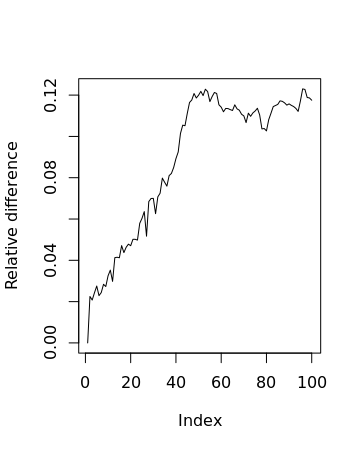
\includegraphics[width=0.19\textwidth]{wdbc_RD.png}}
	\subfloat[Waveform]{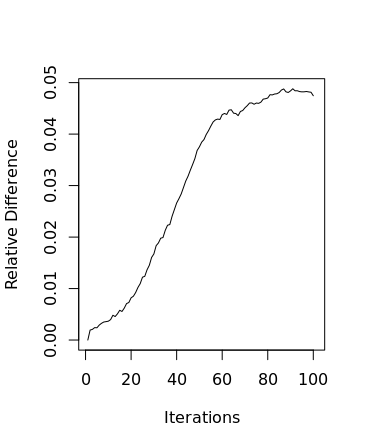
\includegraphics[width=0.19\textwidth]{waveform_RD2.png}}
	\subfloat[Spambase]{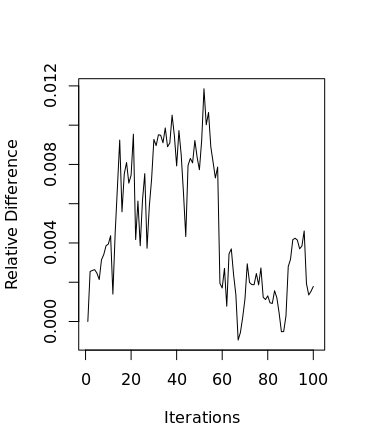
\includegraphics[width=0.19\textwidth]{spambase_RD3.png}}
	\subfloat[Isolet]{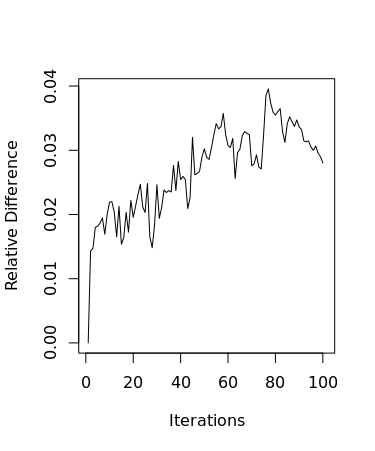
\includegraphics[width=0.19\textwidth]{isolet_RD2}}
	\subfloat[VHR Strasbourg]{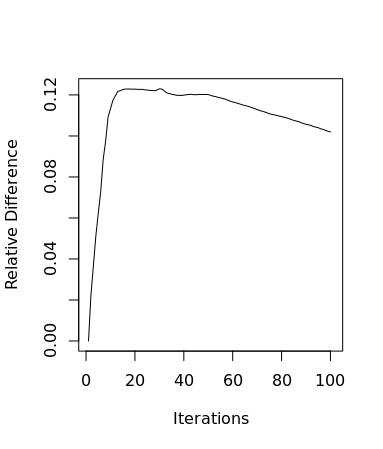
\includegraphics[width=0.19\textwidth]{vhr_RD}}
	\caption{Différences relatives des critères pondérés avec et sans optimisation des $\beta$ tout au long du processus d'apprentissage}
\label{fig:relative_difference}
\end{figure}

\begin{figure}[!h]
	\centering
	\subfloat[WDBC]{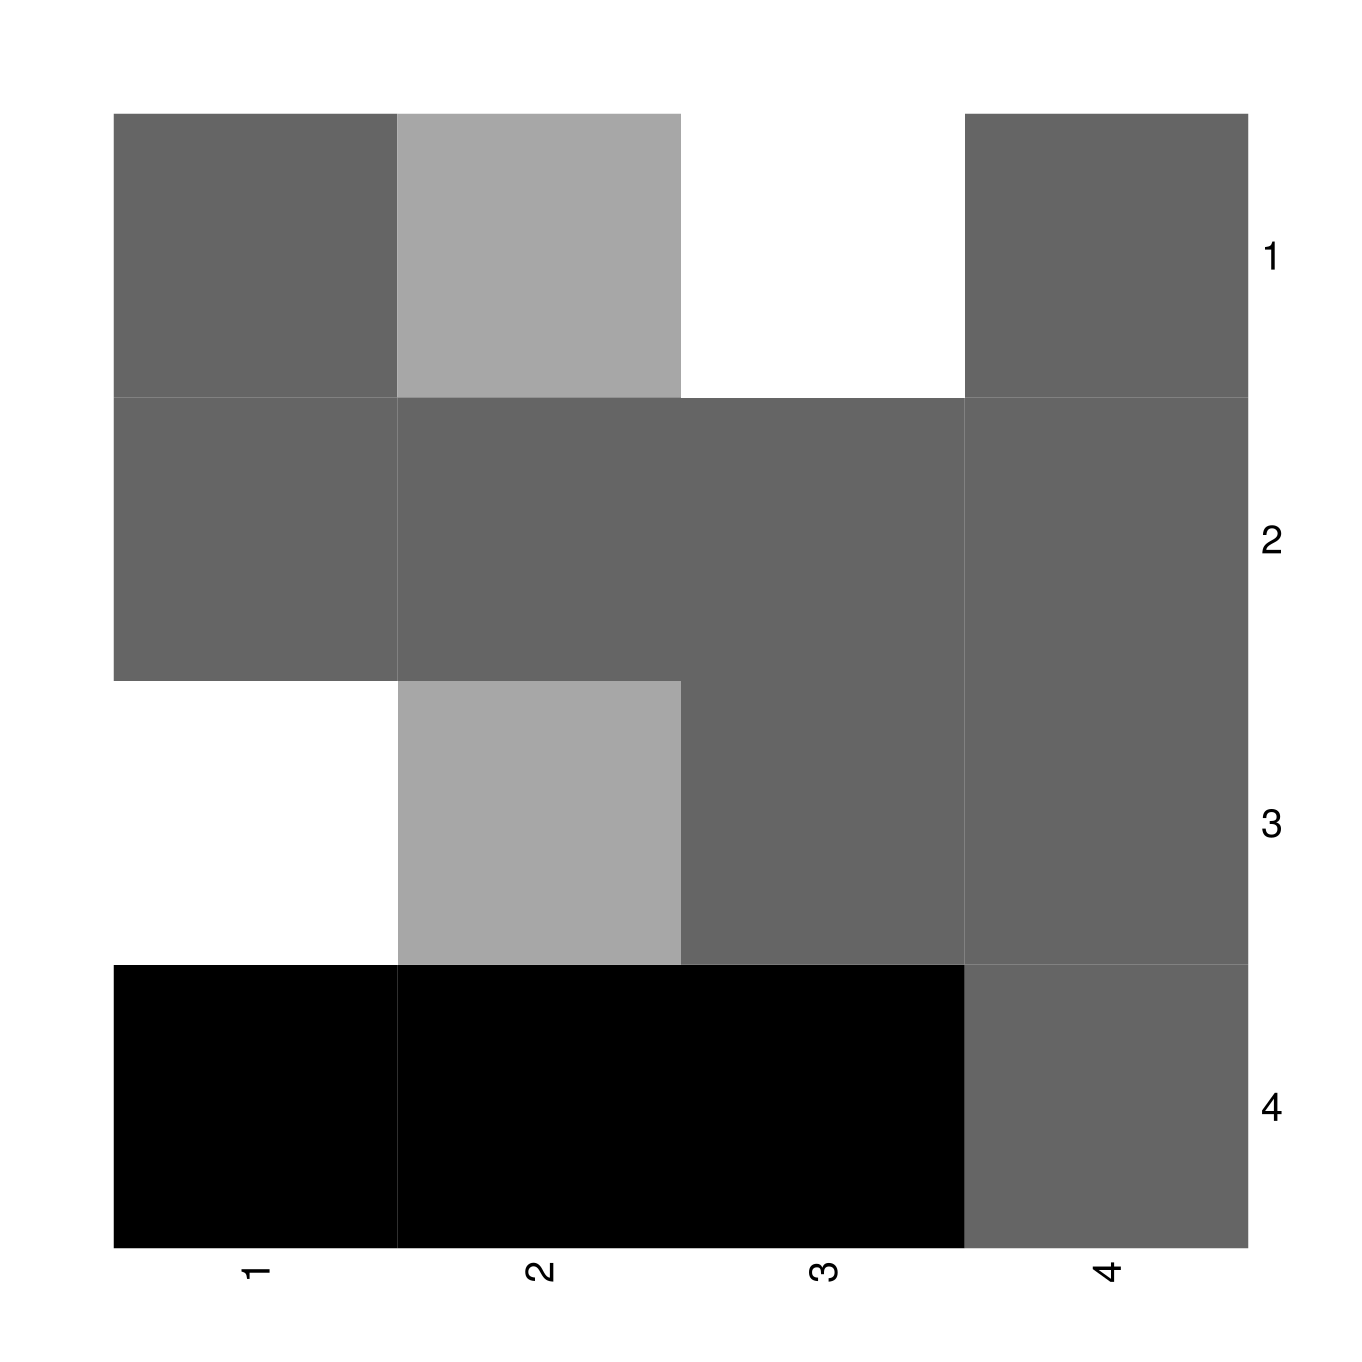
\includegraphics[width=0.19\textwidth]{wdbc_bw}}
	\subfloat[Waveform]{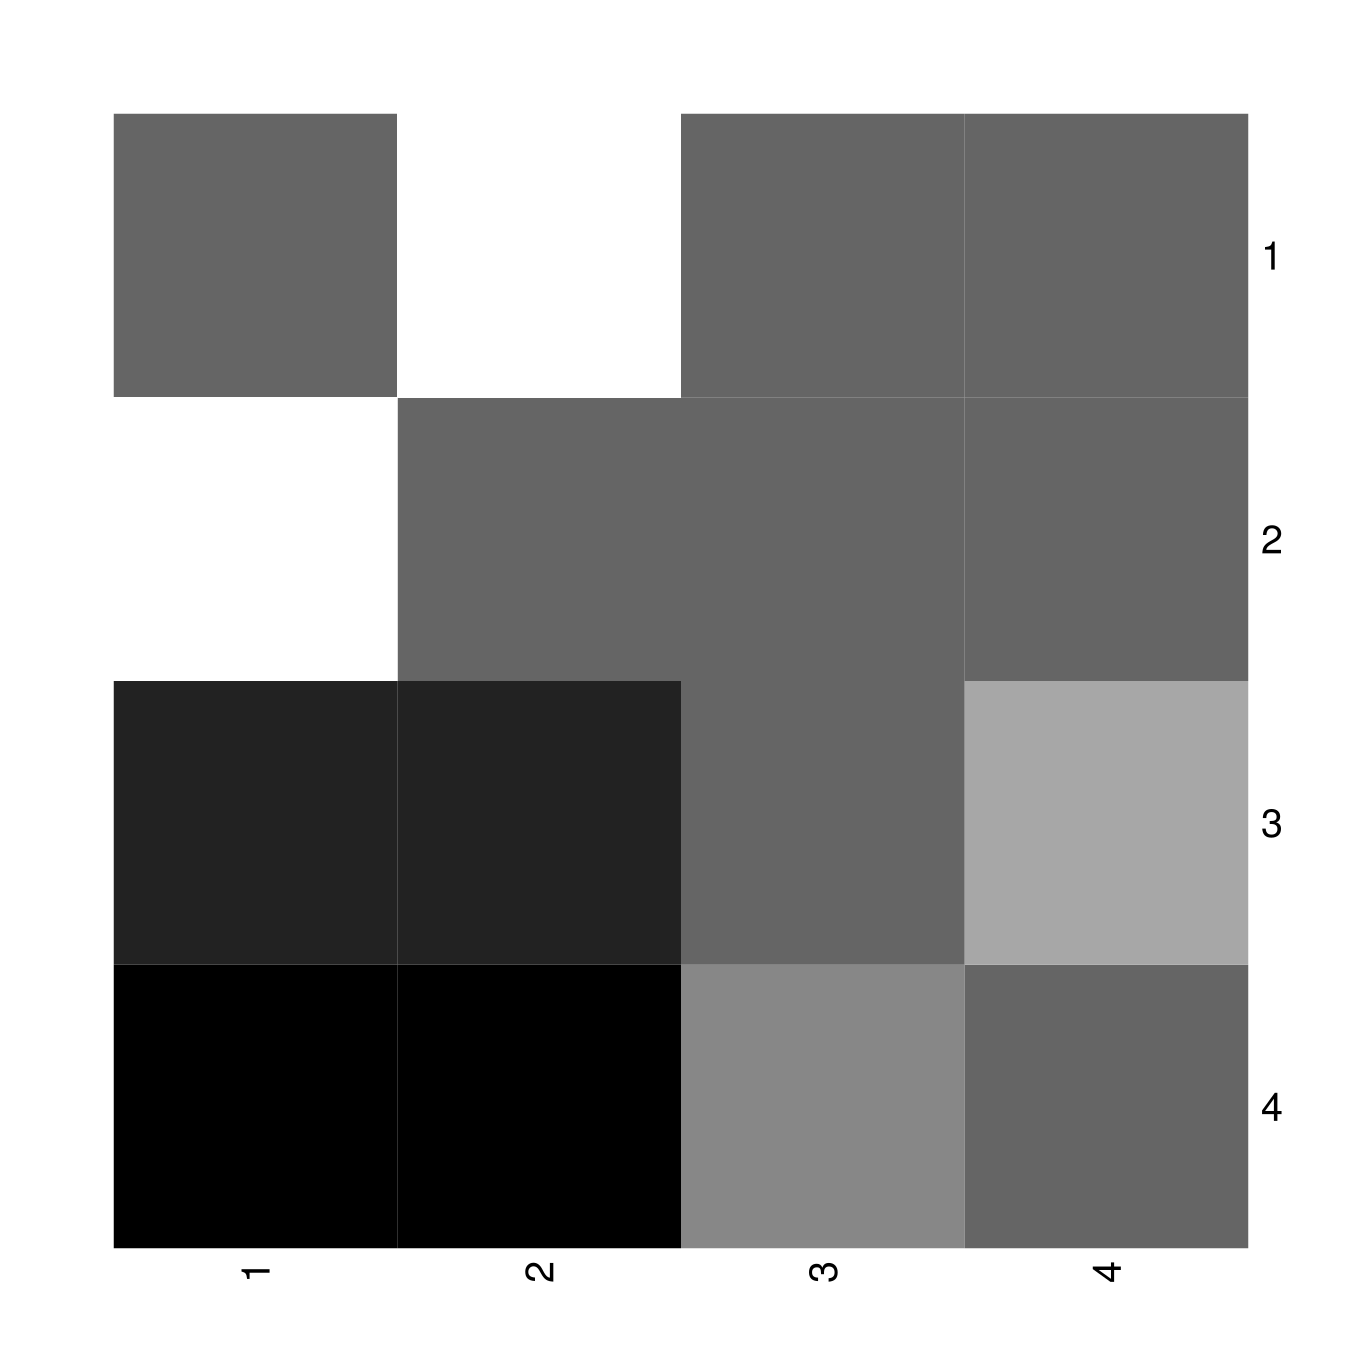
\includegraphics[width=0.19\textwidth]{waveform_bw}}
	\subfloat[Spambase]{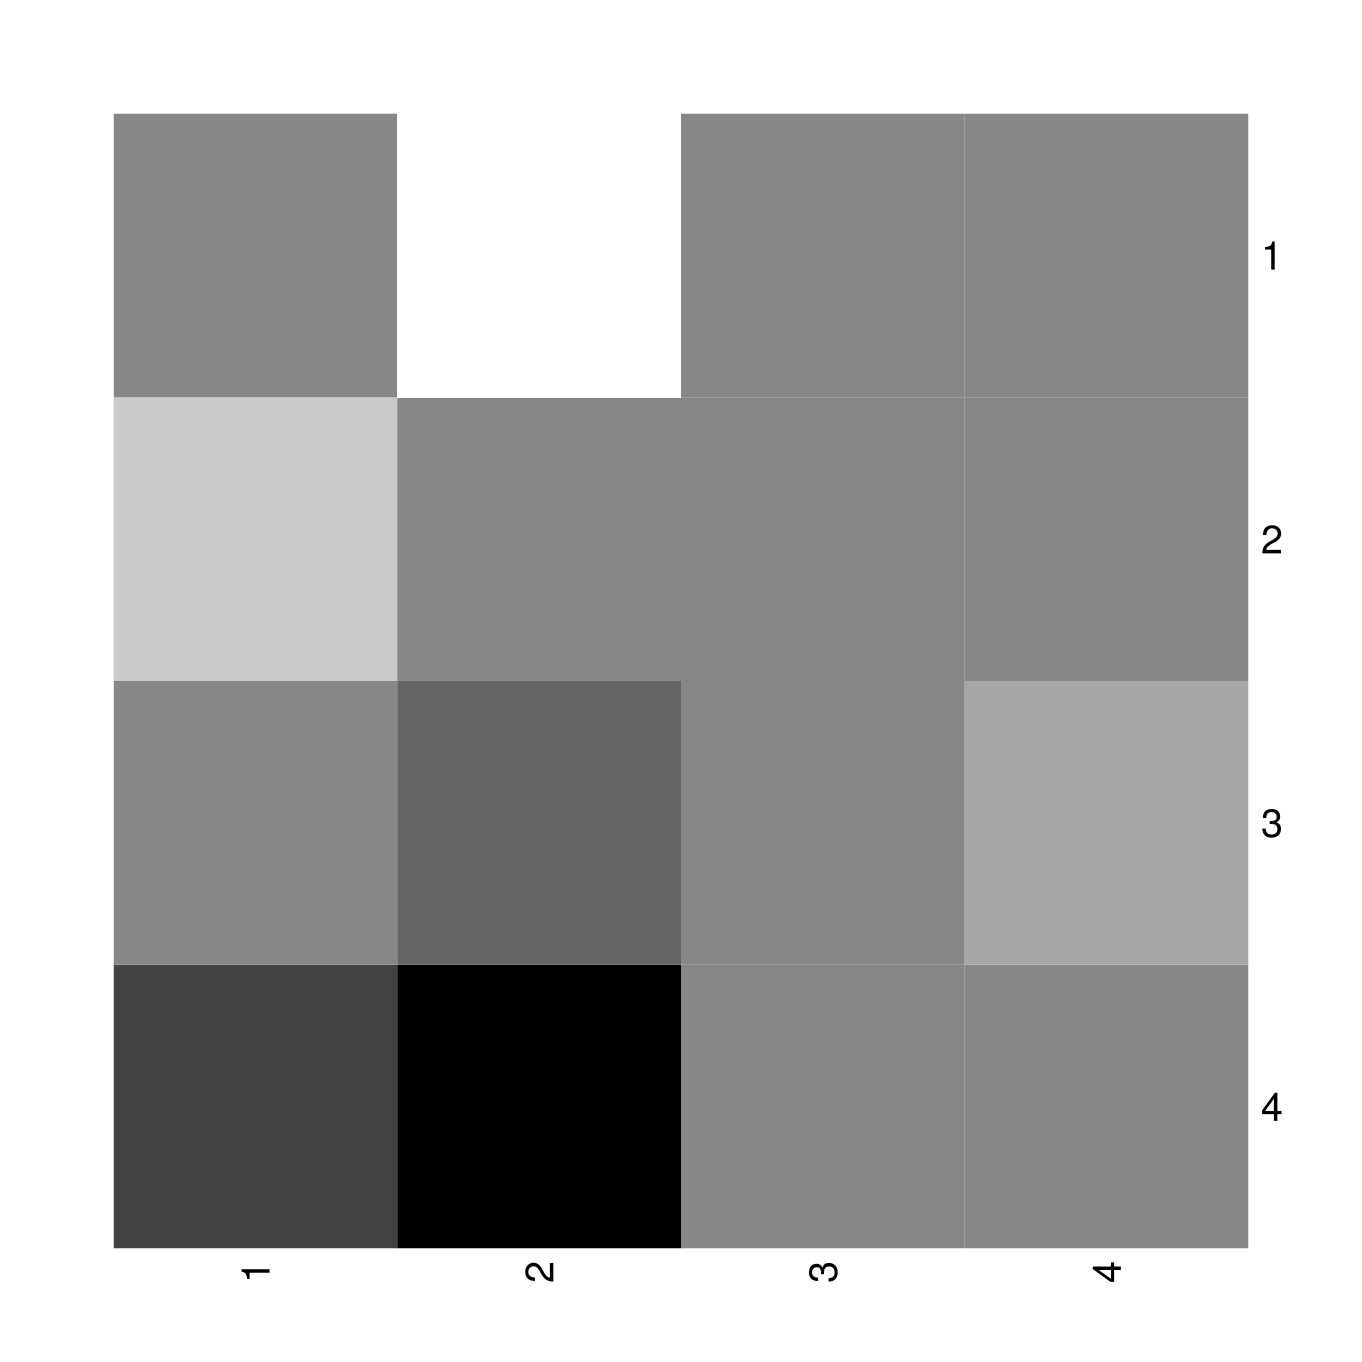
\includegraphics[width=0.19\textwidth]{spambase_bw}}
	\subfloat[Isolet]{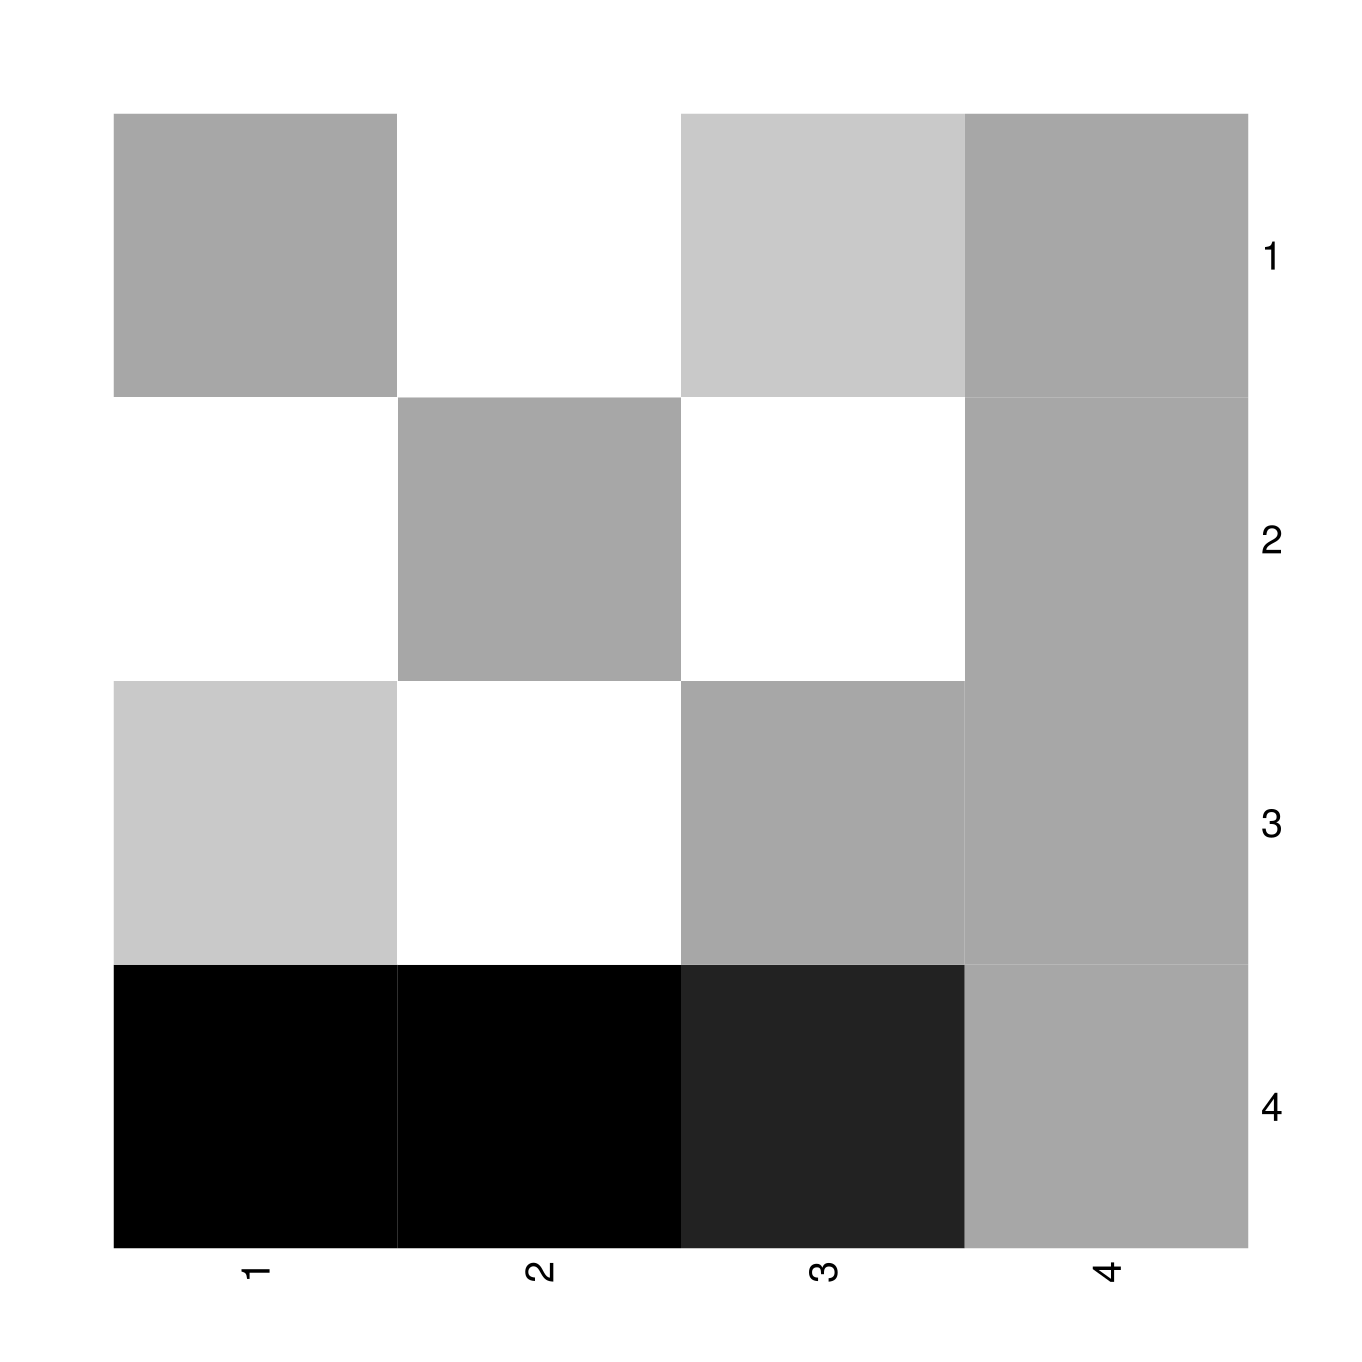
\includegraphics[width=0.19\textwidth]{isolet_bw}}
	\subfloat[VHR Strasbourg]{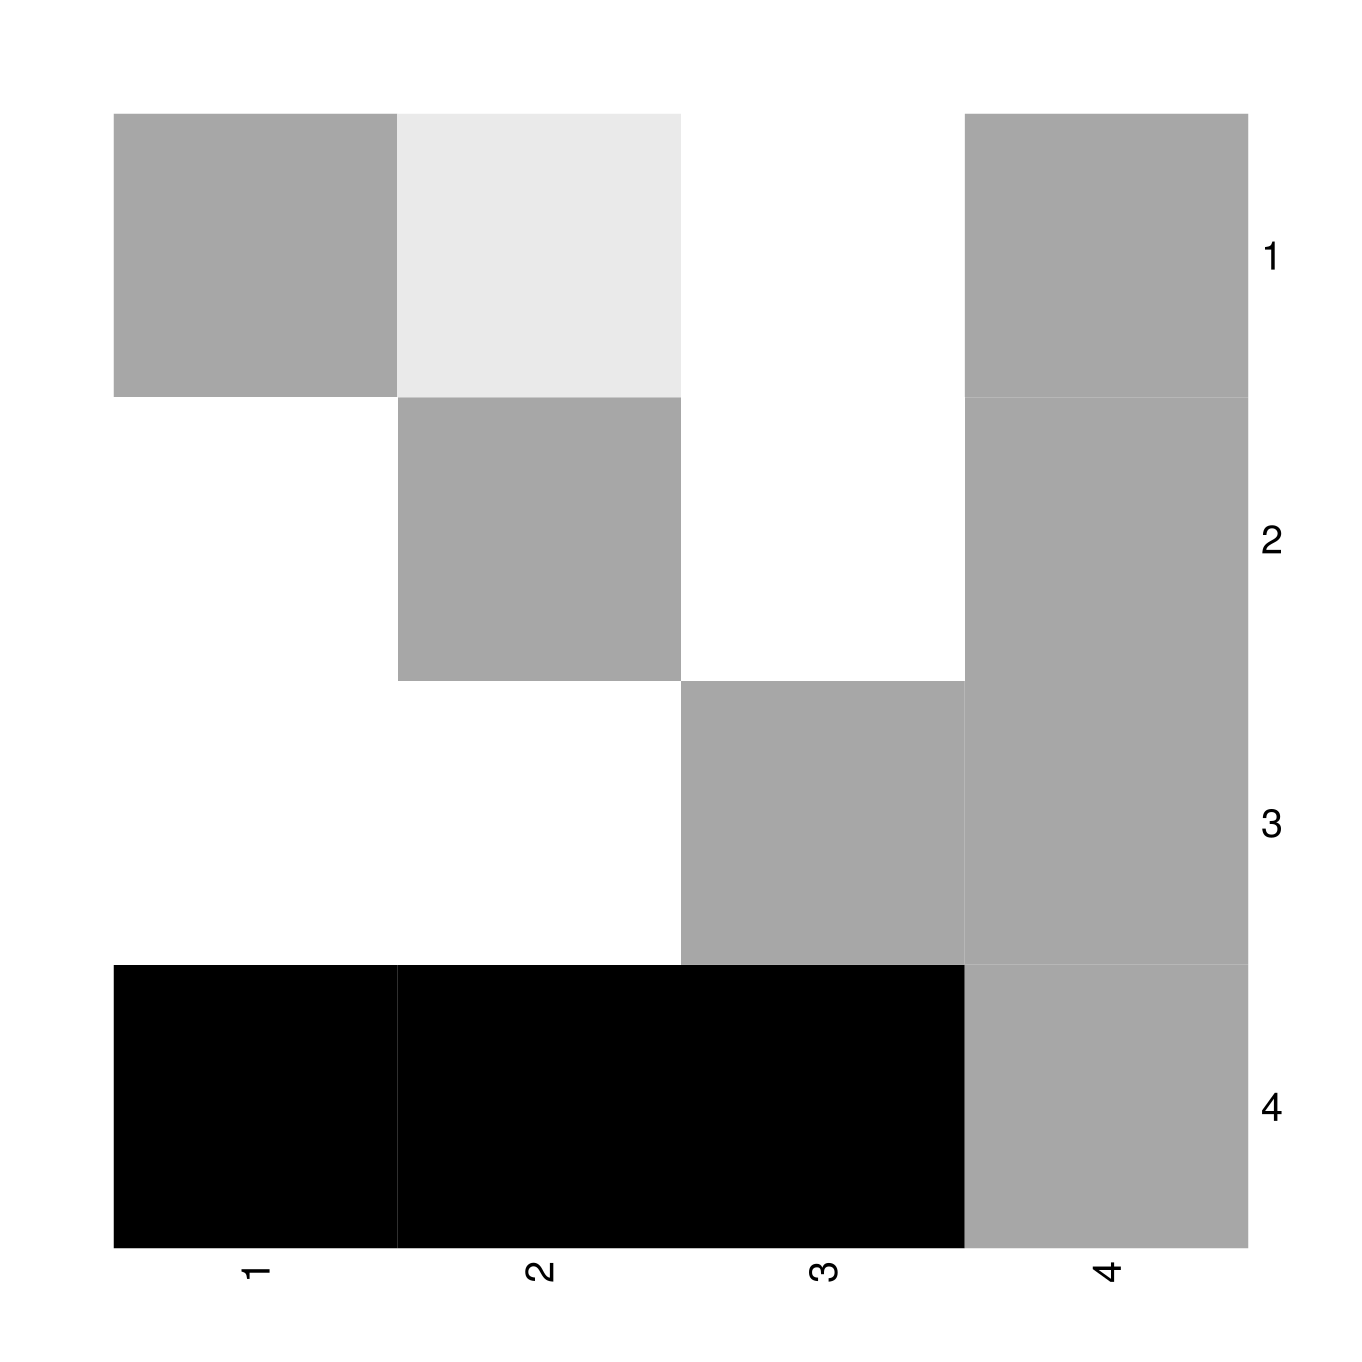
\includegraphics[width=0.19\textwidth]{vhr_bw}}
	\caption{Heatmap of the $\beta$ matrices for each dataset. Colors go from white (strong collaboration) to black (weak collaboration). The gray color on the diagonal stands for $\beta=1$.}
\label{fig:betas}
\end{figure}

Ces cartes font clairement apparaître l'identification des vues bruitées par notre méthode. Tandis que toutes les vues arrivent à identifier les vues bruitées afin de ne pas prendre en compte leurs résultats, les vues bruitées considèrent les vues non bruitées indépendamment de leurs résultats. On peut aussi noter que les vues non bruitées ne coopèrent pas toujours entre elles. Ainsi pour WDBC, les vues 1 et 3 collaborent exclusivement entre elles, tandis que la vue 2 tire son information des deux vues précédentes.

De plus, comme on peut le voir pour Waveform, les vues similaires ont tendance à se regrouper entre elles. Les deux vues bruitées collaborent exclusivement entre elles, de même que les deux vues non bruitées.

En conclusion, notre méthode permet d'adapter dynamiquement les communications inter-vues pour du clustering collaboratif à l'aide de coefficients scalaires représentant l'importance qu'une vue accorde à l'information d'une de ses paires. L'efficacité de la méthode ainsi que sa capacité à regrouper les vues similaires sont démontrées par les expériences. Dans la section suivante, nous présentons les résultats obtenus sur l'adaptation du clustering collaboratif afin de permettre son apprentissage en ligne. Cet axe a été étudié afin d'explorer l'impact qu'aurait un tel contexte sur les communications inter-vues.

\subsection{Cartes auto adaptatrices incrémentales appliquées au clustering collaboratif}

Dans cette section, nous présentons les contributions suivantes:
\begin{itemize}
    \item La définition d'une méthode permettant d'apprendre des Cartes Auto Adaptatrices (CAA) en ligne (au cours du temps).
    \item L'adaptation d'une méthode de clustering collaboratif permettant de tenir compte des modifications apportées aux Cartes Auto Adaptatrices.
    \item Le développement et la présentations de résultats empiriques montrant l'efficacité de notre méthode.
\end{itemize}

L'adaptation du clustering collaboratif à l'apprentissage en ligne a nécessité l'adaptation du modèle utilisé localement pour obtenir une première version des clusterings locaux. Nous avons choisi les Cartes Auto Adaptatrices car elles constituent un modèle couramment rencontré dans la littérature sur le clustering collaboratif~\cite{grozavu2010topological,ghassany2012collaborative,rastin2015collaborative}.

Bien que plusieurs versions en ligne des Cartes Auto Adaptatrices ont été proposées dans la littérature~\cite{deng2000esom,paplinski2012incremental}, toutes se basent sur des modifications topologiques des cartes originales afin de les adapter à l'évolution des données. Ce type de changement n'est pas permi initialement par le clustering collaboratif, du fait des comparaisons qui sont susceptibles d'être faites neurones à neurones entre les cartes. Plutôt que d'adapter les règles du clustering collaboratif afin de permettre ce genre de modifications, nous avons choisi de définir une nouvelle version en ligne de ces cartes pour ensuite l'adapter au clustering collaboratif.

La modification de ces cartes se base sur la modification de la fonction de température permettant de définir le voisinage influencé par la modification de chaque neurone. Cette fonction est normalement dépendante du temps, comme présenté dans la formule suivante:

\begin{equation}
\lambda(t) = \lambda_{\max}{\Big(\frac{\lambda_{\min}}{\lambda_{\max}}\Big)}^{\frac{1}{t}}
\end{equation}

    avec $\lambda_{\max}$ et $\lambda_{\min}$ deux constantes définissant respectivement les températures initiale et finale du modèle. Lorsque la carte est dite ``chaude'', la modification d'un neurone va impacter un large voisinage, c'est l'étape initiale durant laquelle la carte s'adapte grossièrement aux données. Plus l'apprentissage va avancé, plus la carte va se ``refroidir'', pour arriver à de petites valeurs de $\lambda$. Durant cette phase, la carte adaptera plus localement l'emplacement de ces neurones. L'avantage de cette méthode par rapport à une méthode telle que K-means est que l'on conserve une dimension topologique entre les clusters, alors que les centroids de K-means sont indépendants les uns par rapport aux autres.

Afin de s'affranchir de la dépendance temporelle de la fonction de température et afin de la rendre réactive aux éventuels changement dans la distribution des données, nous avons défini la fonction de température $\widetilde{\lambda}$ suivante:

	\begin{equation}
        \widetilde{\lambda}(B, W) = \frac{1}{N_{batch}}\sum_{i=1}^{N_{batch}}\|x_i - \omega_{\chi(x_i)}\|_2
	\end{equation}

    avec $B$ le batch des $N_{batch}$ dernières données arrivées, $W$ l'ensemble des neurones de la carte et $\chi$ la fonction qui a un point associe l'indice du neurone $\omega$ le plus proche de la carte.
    Cette fonction présente le double avantage de ne pas être dépendante du temps tout en s'adaptant à l'état actuel des données: si en moyenne les données sont loins de la carte, la température sera élevée car l'ensemble de la carte aura besoin d'être adaptée. À l'inverse, si les données sont proches de leurs neurones respectifs, la température sera faible car seules des modifications locales des neurones seront nécessaires.

    Cette modification a été inclue dans les équations régissant le comportement du clustering collaboratif afin de le rendre utilisable en ligne. Dans un soucis de concision, le détail des formules n'est pas précisé ici.

    Afin d'attester de l'efficacité de notre méthode, nous avons effectuer des apprentissages sur plusieurs jeux de données: Spam base, Waveform, WDBC et Isolet. Pour chaque jeu de donnée, nous avons regardé quelle était l'erreur de quantification moyenne par vue avec et sans utilisation du clustering collaboratif online. L'erreur de quantification est définie par l'erreur quadratique moyenne entre les individus du batch et leurs neurones les plus proches.

    Les résultats obtenus sont présentés dans le tableau~\ref{tab:tab1}.

	\begin{table}[!h]
        \caption{Erreur de quantification moyenne pour chaque base de donnée. Les nombres en gras sont les plus petits pour chaque ligne}
		\begin{center}
\begin{tabular}{cccc}
                           & Vue & CAA Incrémentales & \begin{tabular}[c]{@{}c@{}}Clustering Collaboratif\\Incrementale\end{tabular} \\ \midrule
\multirow{3}{*}{Spam Base} & 1    & 0.31            & \textbf{0.26}                                                                  \\
                           & 2    & \textbf{0.18}   & 0.19                                                                           \\
                           & 3    & 0.18            & \textbf{0.16}                                                                  \\ \midrule
\multirow{3}{*}{Waveform}  & 1    & \textbf{0.18}   & 0.23                                                                           \\
                           & 2    & \textbf{0.17}   & 0.19                                                                           \\
                           & 3    & \textbf{0.24}   & 0.30                                                                           \\ \midrule
\multirow{3}{*}{WDBC}      & 1    & \textbf{0.19}   & 0.19                                                                           \\
                           & 2    & \textbf{0.16}   & 0.19                                                                           \\
                           & 3    & 0.20            & \textbf{0.16}                                                                  \\ \midrule
\multirow{3}{*}{Isolet}    & 1    & 2.15            & \textbf{1.27}                                                                  \\
                           & 2    & 2.84            & \textbf{1.38}                                                                  \\
                           & 3    & 2.85            & \textbf{1.37}                                                                 \\ \midrule
\end{tabular}
		\end{center}
\label{tab:tab1}
	\end{table}

    Ces résultats indiquent que pour toutes les bases de données sauf Isolet, la carte auto adaptatrice en ligne que nous avons proposée obtient des scores avoisinnant ceux de la version avec clustering collaboratif. C'est un point utile car l'utilisation du clustering collaboratif peut éventuellement réduirel a qualité des résultats obtenus localement du fait de la recherche d'un concensus global. Pour la cas particulier d'Isolet, les meilleurs résultats pour la méthode collaborative peuvent être expliqués par la limitiation de l'impact des données bruitées (96\% des données) grâce au clustering collaboratif.

    Nous avons de même étudié l'impact de notre méthode sur l'apprentissage au cours du temps d'un modèle collaboratif. Pour se faire, nous avons comparé les valeurs des puretés obtenus d'une part par notre méthode de clustering collaboratif online, et d'autre part par une méthode de clustering classique pour laquelle nous prenions chaque itération comme une unité de temps. Les résultats obtenus sont présentés sur la Figure~\ref{fig:isom}. La pureté d'un neurone est égale à la fraction d'individus qui lui sont rattachés et qui appartiennent à la classe la plus représentée sur ce noeud. Par extension, la pureté d'une carte est égale à la pureté moyenne de ses noeuds.

				\begin{figure}[!h]
					\centering
                    \subfloat[$N_{batch}=10$, View 1]{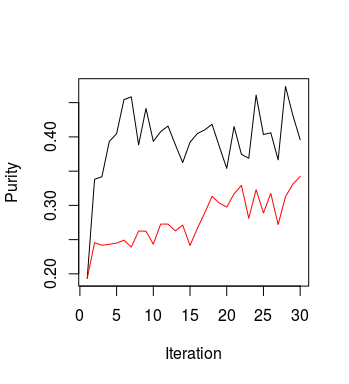
\includegraphics[width=0.33\textwidth, trim= 0 0.5cm 1cm 2cm, clip]{img/11.png}\label{img1}}
                    \subfloat[$N_{batch}=10$, View 2]{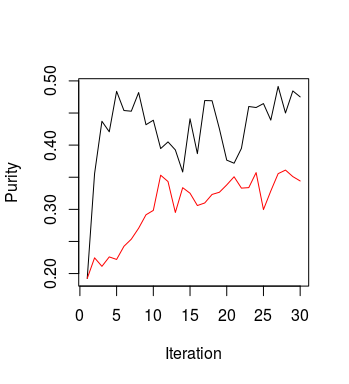
\includegraphics[width=0.33\textwidth, trim= 0 0.5cm 1cm 1.73cm, clip]{img/22.png}\label{img2}}
                    \subfloat[$N_{batch}=10$, View 3]{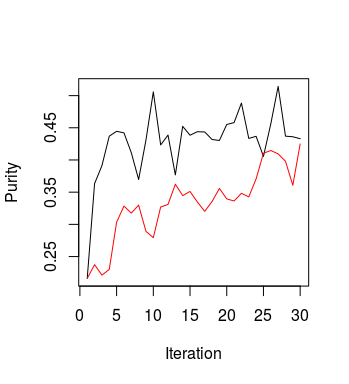
\includegraphics[width=0.33\textwidth, trim= 0 0.5cm 1cm 2cm, clip]{img/33.png}\label{img3}}\\
                    \subfloat[$N_{batch}=3$, View 1]{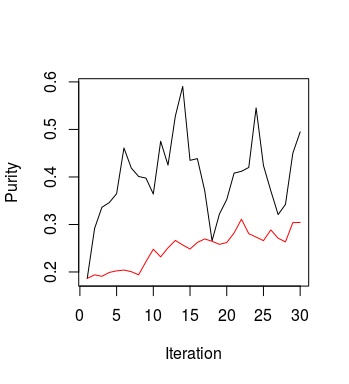
\includegraphics[width=0.33\textwidth, trim= 0 0.5cm 1cm 1.9cm, clip]{img/p1.png}\label{img4}}
                    \subfloat[$N_{batch}=3$, View 2]{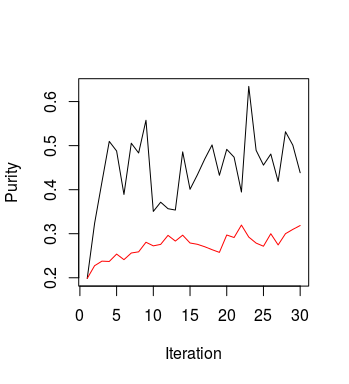
\includegraphics[width=0.33\textwidth, trim= 0 0.5cm 1cm 2cm, clip]{img/p2.png}\label{img5}}
                    \subfloat[$N_{batch}=3$, View 3]{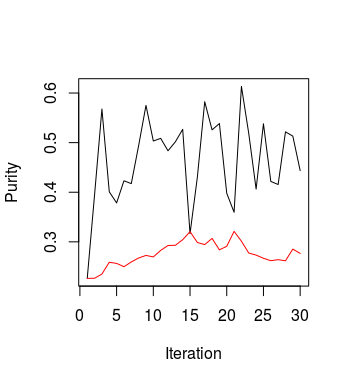
\includegraphics[width=0.33\textwidth, trim= 0 0.5cm 1cm 2cm, clip]{img/p3.png}\label{img6}}
                \caption{Évolution des puretés for le jeu de données Isolet. Les lignes rouges représentes les CAA incrémentales tandis que les lignes noires représentent les CAA collaboratives. Chaque itération correspond à l'arrivée d'une nouvelle donnée}
\label{fig:isom}
				\end{figure}


    Ces figures font apparaître une meilleure pureté pour notre méthode par rapport à la méthode classique dans la première phase de l'apprentissage. À l'adaptation en temps réel qui est faite sur la fonction de température, permettant d'obtenir de meilleurs résultats plus rapidement qu'avec une méthode classique. On peut de plus remarquer l'influence du paramère $N_{batch}$ sur l'apprentissage: une valeur plus faible implique une variance plus importante de la pureté au cours du temps. Ce point se comprend intuitivement par le fait que lorsque $N_{batch}$ est faible, le système dispose de peu d'informations pour adapter ses neurones, ce qui implique nécessairement une grande variabilité suivant l'échantillon de données en cours de traitement.

    En conclusion, nous avons présenté dans cette section une méthode permettant d'effectuer un apprentissage en ligne des cartes auto adaptatrices sans utiliser de modification topologique. Cette méthode a ensuite été adaptée au clustering collaboratif, puis son efficacité a été présenté sur différents jeux de données. L'influence du nombre de données par échantillon a été étudiée et reliée à la variance des scores obtenus lors de l'apprentissage.

    La section suivante présente un use case différent de celui du clustering traité jusqu'à présent. L'objectif principal de cette thèse étant d'explorer les possibilités offertes par les communications inter-vues dans un contexte collaboratif, nous nous sommes intéressé au problème des données manquantes et aux manières d'y pallier.

\section{Système de reconstruction collaborative}

Les contributions présentées dans cette section sont les suivantes:
\begin{itemize}
    \item Définition d'un nouveau cas d'utilisation dans un contexte d'apprentissage collaboratif: la reconstruction collaborative.
    \item Définition d'un modèle pouvant répondre au problème posé.
    \item Définition d'une nouvelle méthode de pondération permettant de combiner des vecteurs point à point.
    \item Attestation de l'efficacité du modèle au travers d'expériences menées sur divers jeux de données avec identification des limites du modèle et de pistes d'améliorations.
\end{itemize}

Le clustering collaboratif se base sur l'hypothèse que les vues communicantes disposent de suffisamment d'individus en commun pour échanger leurs résultats et les comparer. Cependant en pratique, la récupération de plusieurs bases de données sur un même ensemble d'individus est une chose difficile à mettre en place, et la récupération des données peut entraîner l'apparition de données manquantes. L'idée initiale développée dans cette section a été qu'il était possible d'utiliser l'ensemble des informations disponibles sur le sous ensemble d'individus en commun entre les vues pour inférer les valeurs des individus manquants.

Une représentation de l'architecture de notre méthode est présentée sur la Figure~\ref{fig:sum_base}. Alors que le clustering collaboratif se base sur une correspondance cluster à cluster, la reconstruction collaborative s'appuie elle sur l'inférence de données cibles à partir de données initiales. La difficulté de la mise en pratique de cette idée a motivé l'utilisation de réseaux de neurones, et plus particulièrement de Perceptrons Multi-Couches (aussi appelés Liens, ou Link en anglais), comme liens entre les vues afin de donner une première approximation de l'individu manquant. L'apprentissage de tels réseaux est possible du fait de la présence d'un ensemble d'individus en commun à une paire de vue. En utilisant les descriptions de la vue externe comme entrée et celles de la vue locale comme sortie, il était possible d'effectuer un apprentissage supervisé du réseau.

	\begin{figure}[H]
		\centering
        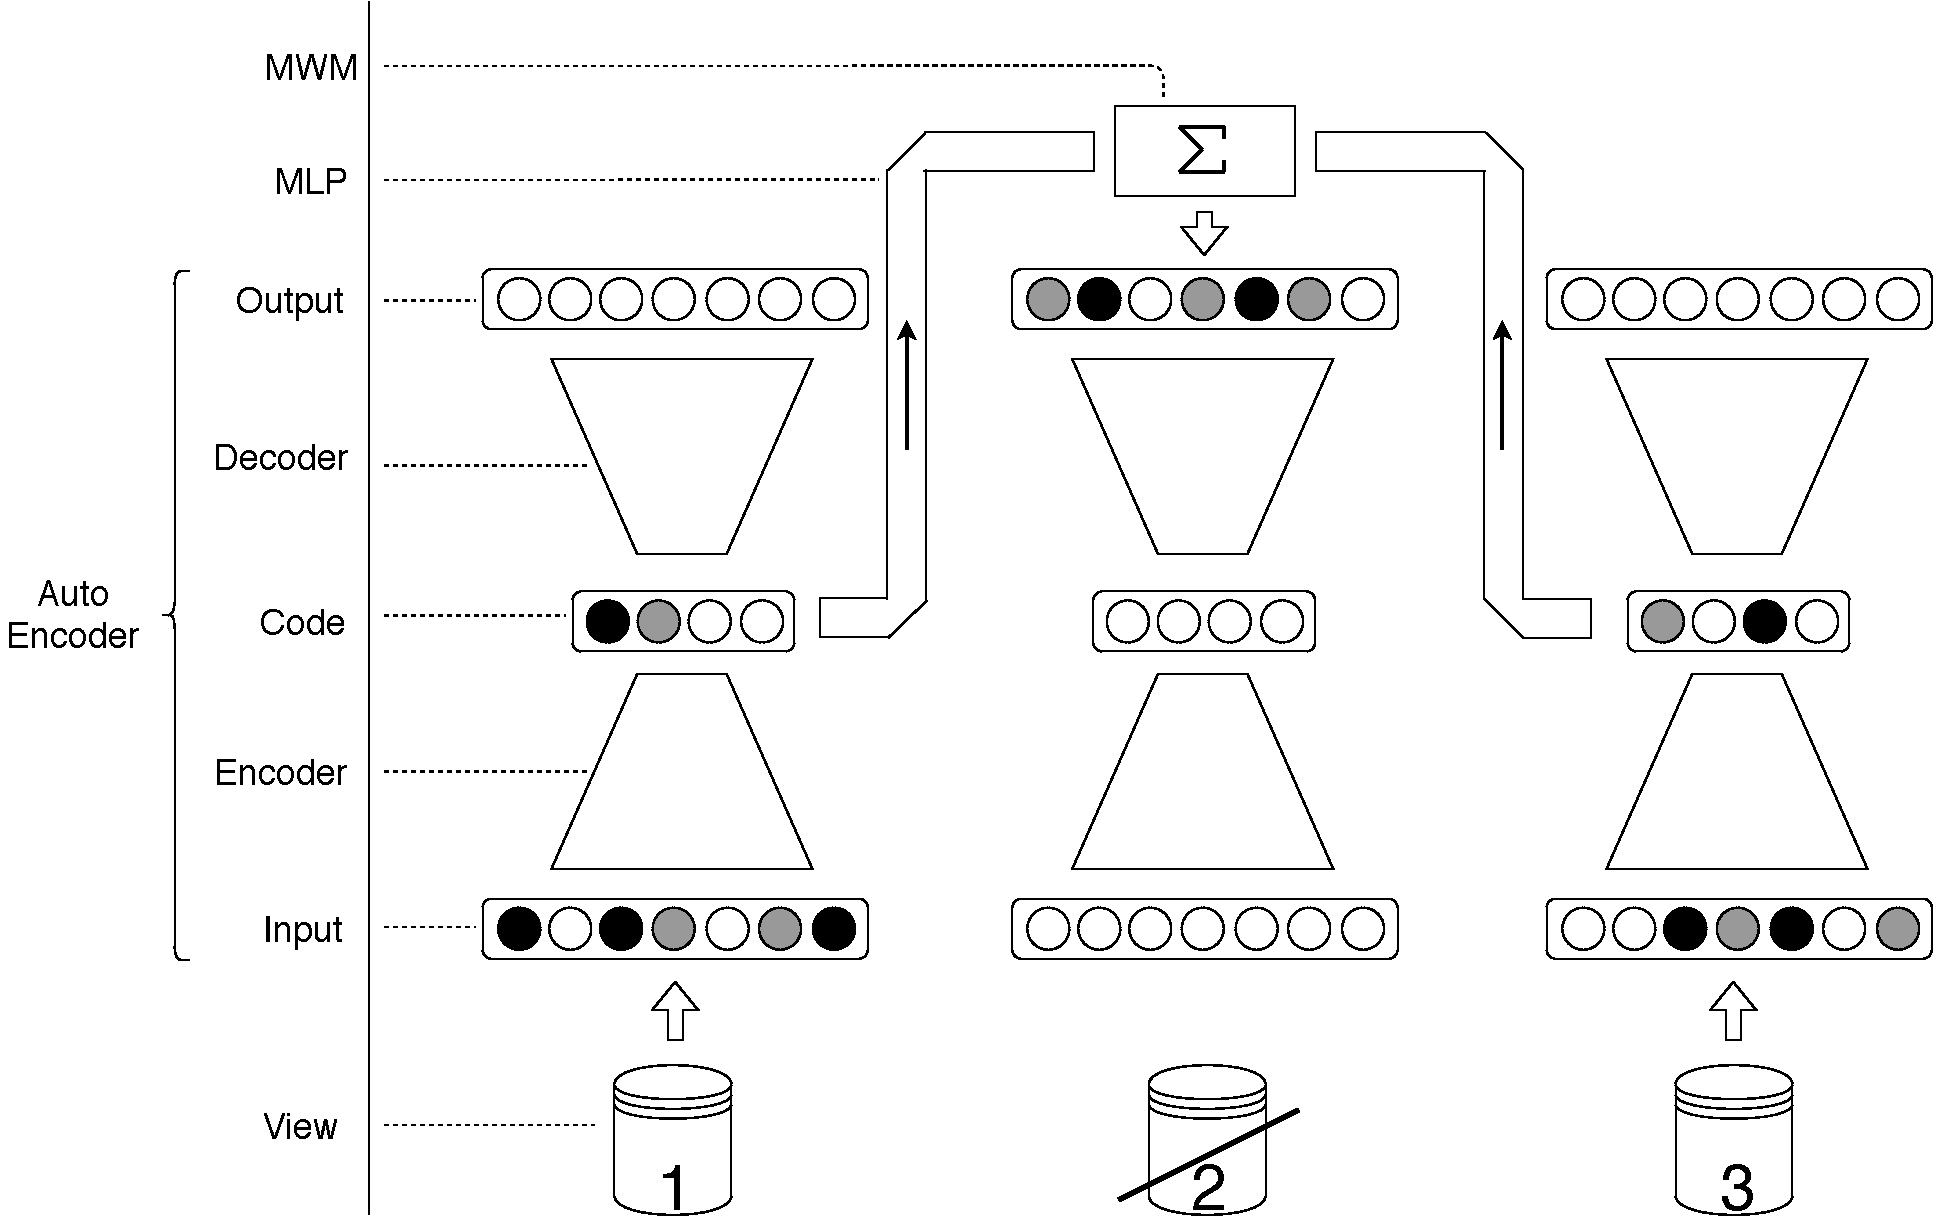
\includegraphics[width=0.8\textwidth]{img/base_system.pdf}
        \caption{Système de recontruction coopérative. Dans cet example, les vues 1 et 3 envoient leur versions codées de l'individu à la vue 2.}
\label{fig:sum_base}
	\end{figure}

    Un autre aspect propre au clustering collaboratif constitue la sécurité qu'il met en place concernant les données en transit: les données originales ne sont jamais transférées d'une vue à une autre. À la place sont transférées soit les identifiants des clusters auxquels appartiennent les individus~\cite{sublime2016collaborative,Sublime2015}, soit des informations utilisées au cours de l'apprentissage comme c'est le cas pour l'apprentissage à l'aide de cartes SOM~\cite{ghassany2012collaborative,maurel2017incremental}. Dans le cas de la reconstruction collaborative, l'utilisation d'un réseau de neurone comme système d'inférence implique nécessairement un codage des données initiales sous la forme d'un vecteur scalaire qui sera utilisé à la place des données originales comme données d'entrée du réseau en charge de l'inférence. Ce codage sous forme de vecteur est assuré dans notre modèle par un auto-encodeur, une catégorie de réseaux de neurones ayant la particularité de reconstruire en sortie les données fournies en entrée~\cite{vincent2008extracting}. 

    Enfin, le dernier composant de notre méthode consiste en une méthode de pondération, que nous avons appelé méthode de pondération par masques, qui permet de combiner l'ensemble des approximations créées à partir des données reçues des vues externes ($N-1$ dans un système à $N$ vues où chaque vue externe aurait une information sur l'individu manquant). L'idée fondamentale de cette méthode consiste en l'utilisation de vecteurs permettant de pondérer des individus point à point (descripteur par descripteur) plutôt que d'utiliser un unique coefficient pondérant l'ensemble de l'individu. En effet, il est facile d'imaginer que pour un individu manquant donné, chaque vue externe permette d'en reconstruire seulement une partie. L'utilisation d'un coeffcient de pondération unique ne permet pas de prendre en compte cette différenciation. Un schéma décrivant le processus de pondération par un ensemble de vecteurs, que nous appelerons désormais masques, est présenté sur la Figure~\ref{fig:sum_mwm}. Les valeurs des masques sont entraînées au préalable afin de mieux correspondre à chaque vue, et chaque vue possède $N-1$ masques, un par vue externe.

	\begin{figure}[H]
		\centering
		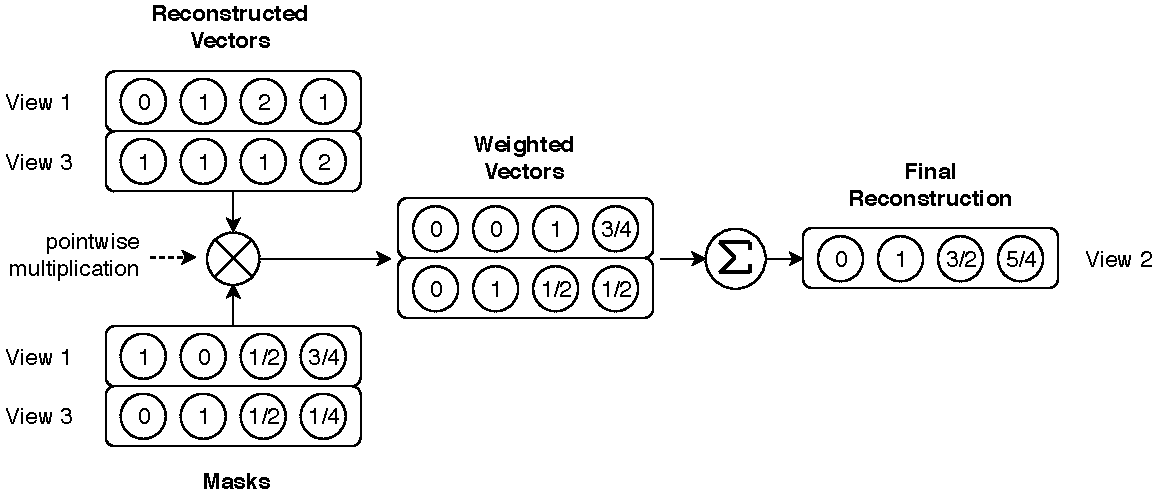
\includegraphics[width=\textwidth]{img/mwm.pdf}
        \caption{La méthode de pondération par masques. La vue 2 possède les individus inférés à l'aide des informations des vues 1 et 3, et elle utilise ses masques entraînés au préalable afin d'obtenir le résultat pondéré final.}
\label{fig:sum_mwm}
	\end{figure}

    L'idée générale de la méthode d'apprentissage consiste simplement en une descente de gradient sur un critère défini comme la distance entre l'individu cible et sa version reconstruite à l'aide des réseaux de neurones et de notre méthode de pondération. Une seconde méthode itérative a été proposée et démontrée analytiquement en annulant le gradient précedemment obtenu et en mettant à jour les poids des masques de manières itérative.\\

    Concernant l'apprentissage du système dans sa globalité, il peut être effectué séquentiellement:
    \begin{enumerate}
        \item Chaque vue entraîne de manière indépendante un auto-encodeur en charge de chiffrer les données originales.
        \item Chaque vue encode l'ensemble de sa base de donnée d'apprentissage et envoie le résultat à ses paires
        \item Chaque vue entraîne $N-1$ perceptrons multi-couches, 1 par vue externe, en mettant en correspondance les individus chiffrés et les individus cibles.
        \item Les vues utilisent leurs perceptrons pour inférer les valeurs des individus présents dans la base d'apprentissage, chaque vue possède alors $N-1$ base de données d'individus inférés.
        \item Les poids des masques sont entraînés à l'aide des $N-1$ bases d'individus inférés et des données originales.\\
    \end{enumerate}

    Une fois l'ensemble de ces étapes effecutées pour toutes les vues du problème, la reconstruction d'un individu manquant devient possible.

    Plusieurs tests ont été effectués à l'aide de notre système de reconstruction collaborative:
    \begin{itemize}
        \item Afin de tester l'efficacité du système global, des reconstructions ont été faites et comparées aux versions originales en utilisant l'erreur quadratique moyenne.
        \item Le test suivant a consisté en une classification des individus reconstruits à l'aide de l'algorithme de Random Forest pour tester si la classe prédite correspondait à la classe réelle.
        \item Enfin, la qualité des reconstructions a été testée en remplaçant la méthode de pondération par masque par une simple moyenne. Le but de ce test a été de vérifier l'efficacité de notre nouvelle méthode de pondération.
    \end{itemize}

    Ces tests ont été effectués sur 4 jeux de données différents: WDBC, Multi-Features Digital Dataset (MFDD), Madelon et Cube. Ce dernier est un jeu de donnée artificiel crée spécialement pour tester l'efficacité de notre méthode de pondération. Il est constitué d'un ensemble de 4 groupes de points répartis dans un espace en 3 dimensions. Trois clusters se trouvent à chacune des extrémités des vecteurs de base, le quatrième se trouvant à l'origine de l'espace. Trois vues sont ensuite créées en projetant l'ensemble du jeu de données suivant chacun des trois vecteurs de base. L'intérêt d'une vue ainsi créée est que l'information permettant de reconstruire ses individus est par définition répartie dans les deux vues restantes. Si notre méthode de pondération fonctionne, on peut s'attendre à ce que les masques privilégient une caractéristique spécifique tout en rejetant totalement l'autre.
    
    Un schéma décrivant la pondération par masque et comment elle permet de s'affranchir de caractéristiques mal reconstruites et/ou bruitées peut être trouvé sur la Figure~\ref{fig:sum_process_mwm}.

\begin{figure}[H]
    \centering
    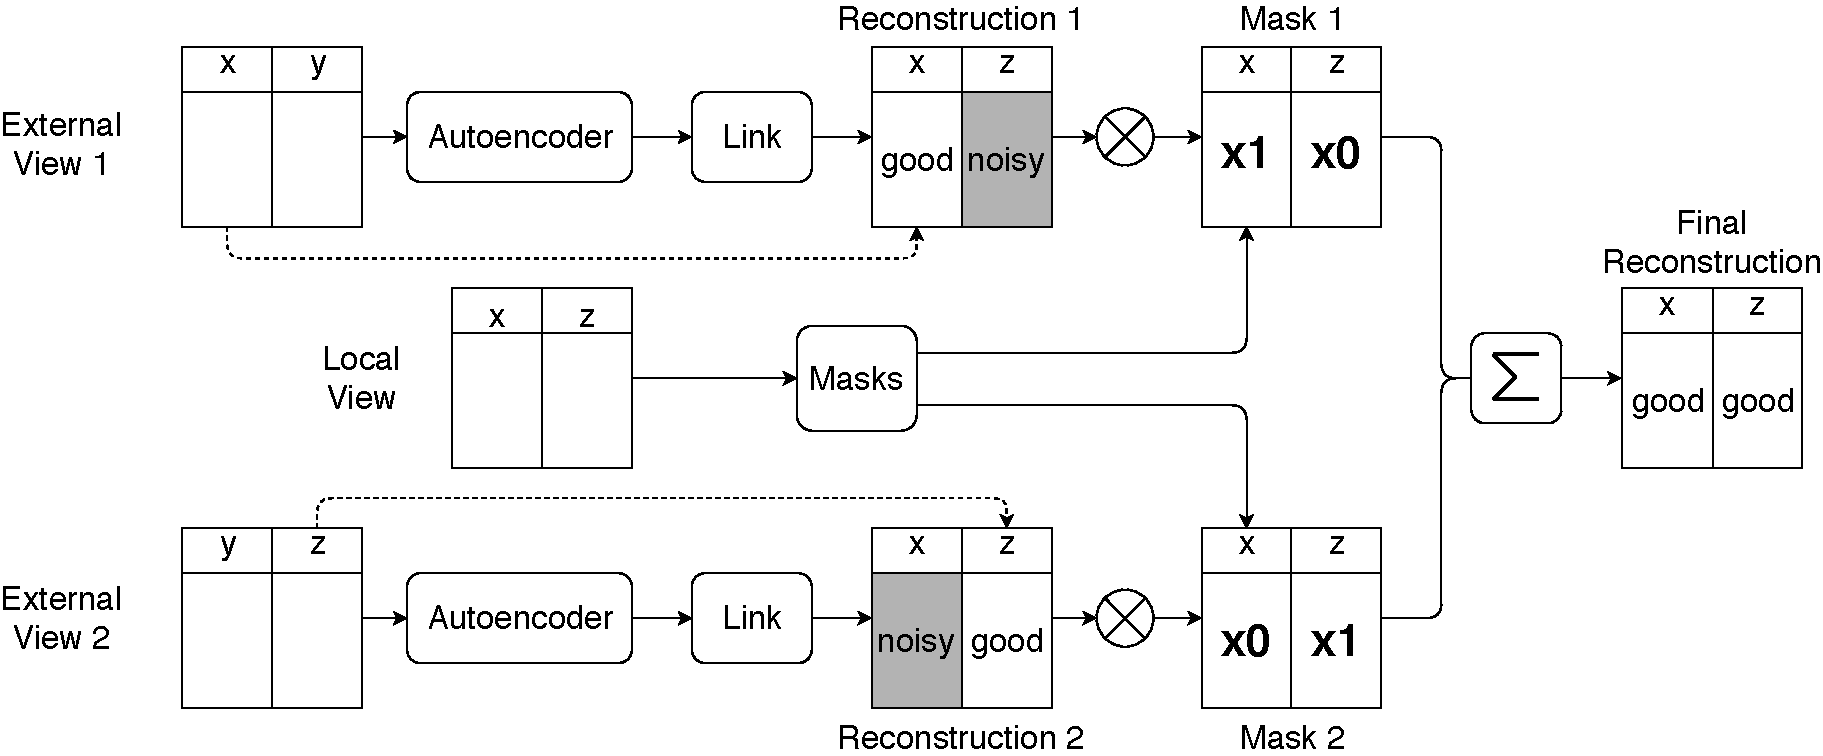
\includegraphics[scale=.38]{img/process_mwm}
    \caption{Combinaison de deux reconstructions partiellement bonnes. Dans cet exemple, chaque vue dispose d'assez d'information pour reconstruire seulement une caractéristique sur les deux dans la vue locale (pointillés). La méthode de pondération par masques favorise les parties les mieux reconstruites de chaque résultat, d'où le $\times 0$ et $\times 1$ dans les masques.}
\label{fig:sum_process_mwm}
\end{figure}

L'utilisation du jeu de données MFDD permet d'obtenir des reconstructions visuelles, permettant d'appréhender plus facilement leurs qualités. La figure~\ref{fig:num_original} montre un échantillon de 10 images avant apprentissage. La figure~\ref{fig:num_reconstructed} présente 10 reconstructions considérées comme de bonnes qualités. Bien qu'il ne s'agisse que d'un résultat purement visuel, la majorité des individus présente une reconstruction de qualité avoisinante à celle des images présentées ci-dessous. Cependant dans certains cas, le système n'a pas été capable d'inférer efficacement les chiffres à reconstruire, ce qui a mené à des reconstructions comme celles présentées en figure~\ref{fig:num_reconstructed_bad}.

\begin{figure}[h]
    \centering
    \subfloat[][]{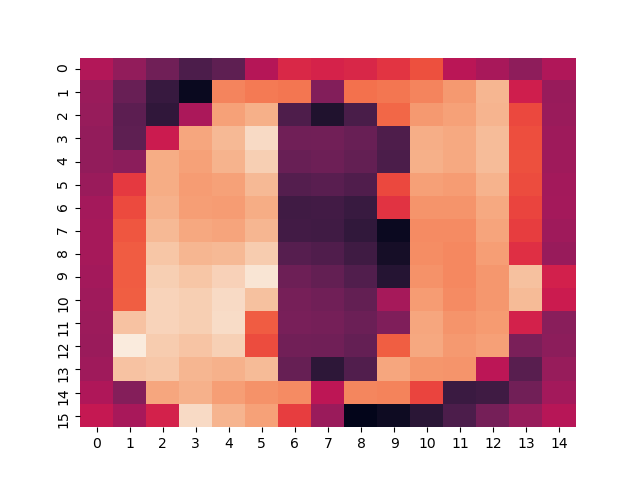
\includegraphics[scale=.07]{img/sample_original/o0}}
    \subfloat[][]{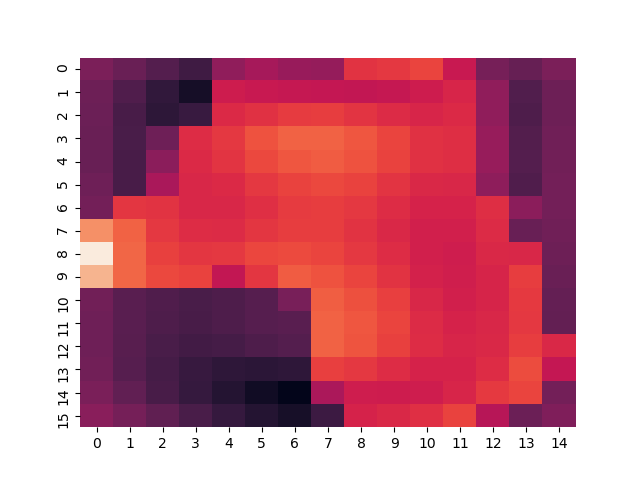
\includegraphics[scale=.07]{img/sample_original/o1}}
    \subfloat[][]{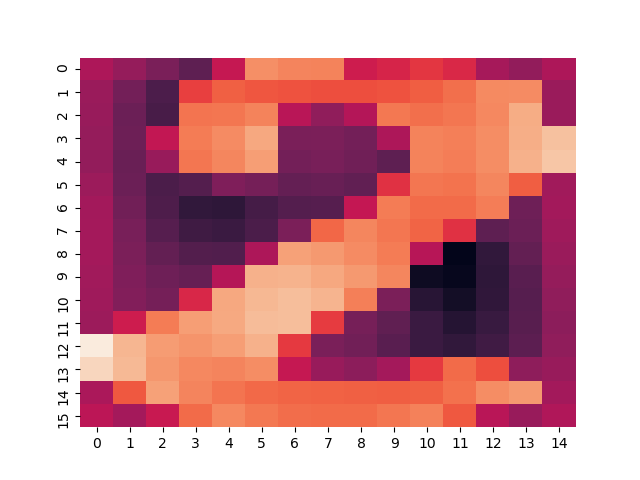
\includegraphics[scale=.07]{img/sample_original/o2}}
    \subfloat[][]{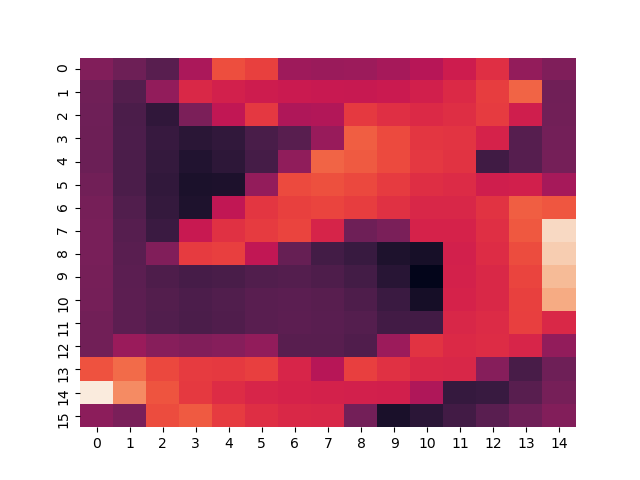
\includegraphics[scale=.07]{img/sample_original/o3}}
    \subfloat[][]{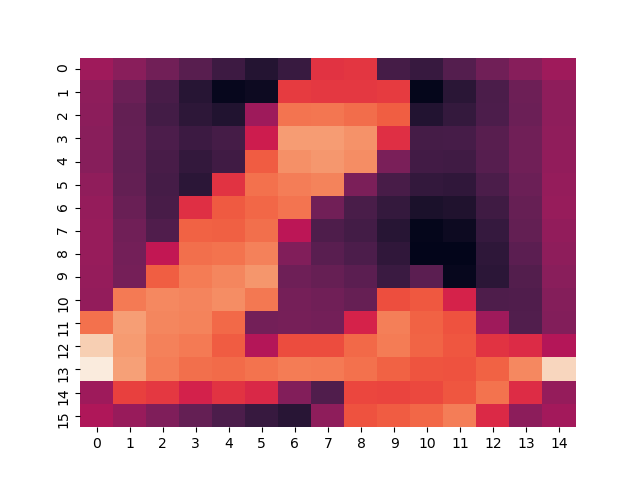
\includegraphics[scale=.07]{img/sample_original/o4}}
    \subfloat[][]{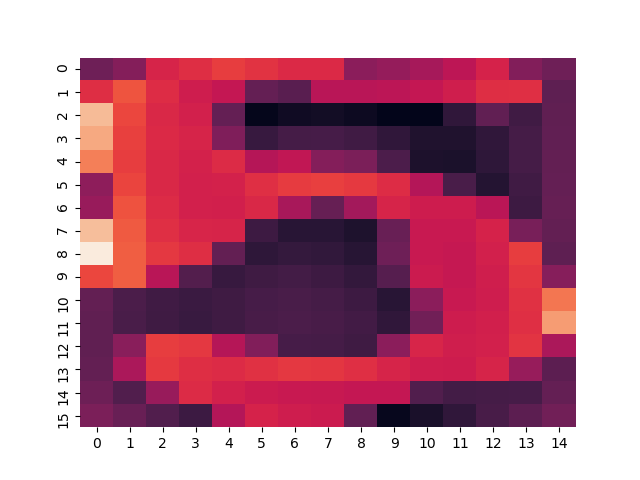
\includegraphics[scale=.07]{img/sample_original/o5}}
    \subfloat[][]{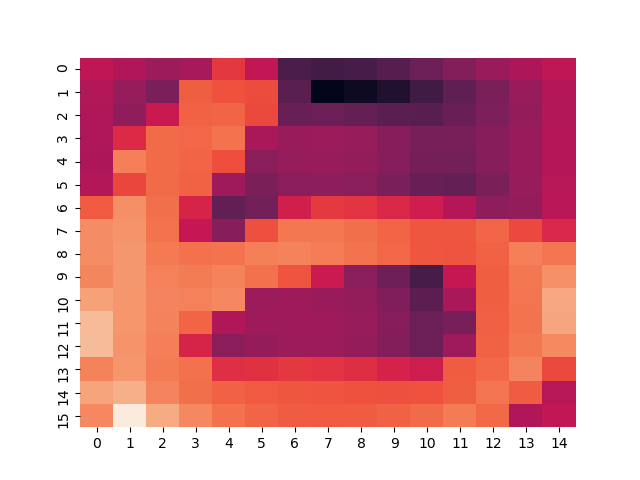
\includegraphics[scale=.07]{img/sample_original/o6}}
    \subfloat[][]{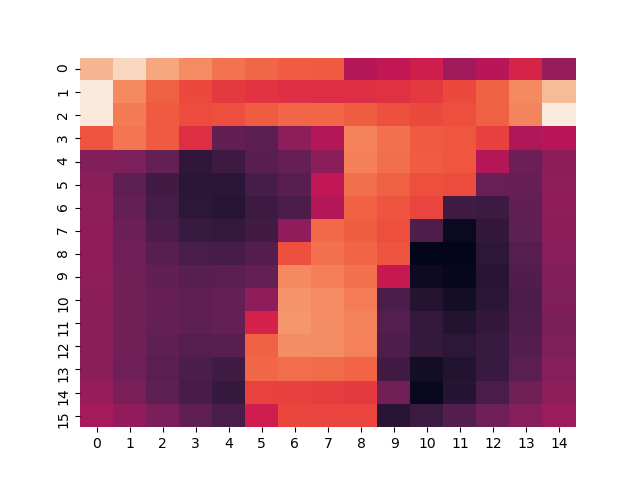
\includegraphics[scale=.07]{img/sample_original/o7}}
    \subfloat[][]{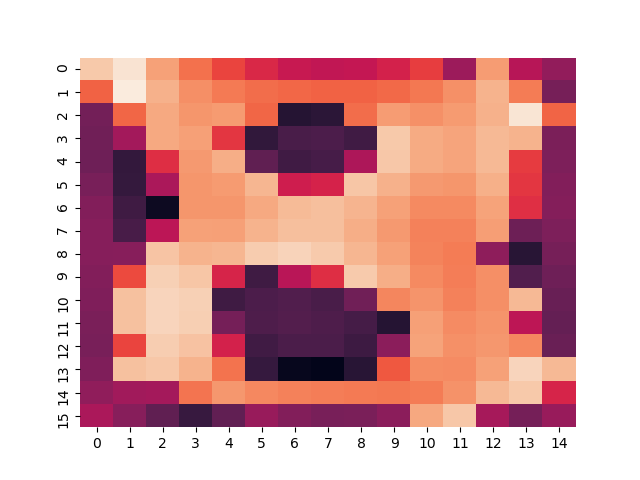
\includegraphics[scale=.07]{img/sample_original/o8}}
    \subfloat[][]{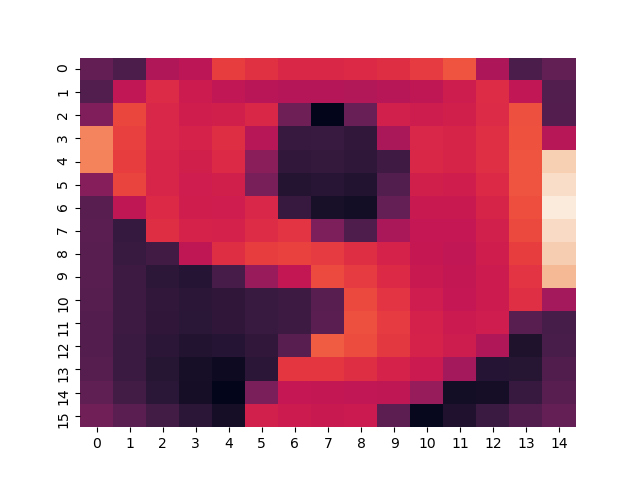
\includegraphics[scale=.07]{img/sample_original/o9}}
    \caption{Échantillon des images disponibles dans le jeu de données MFDD.}
\label{fig:num_original}
\end{figure}

\begin{figure}[h]
    \centering
    \subfloat[][]{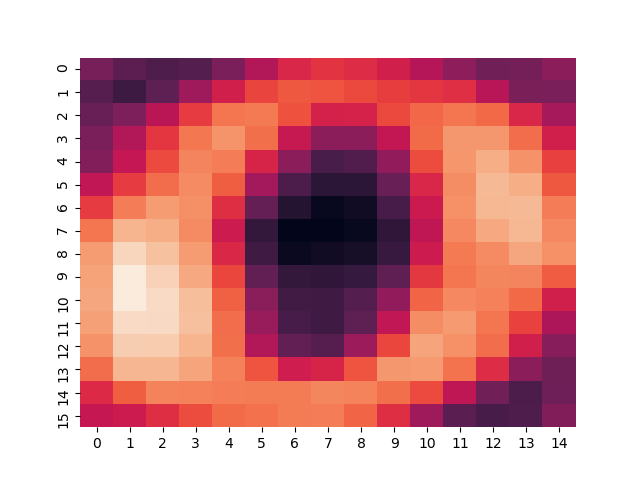
\includegraphics[scale=.07]{img/sample/0}}
    \subfloat[][]{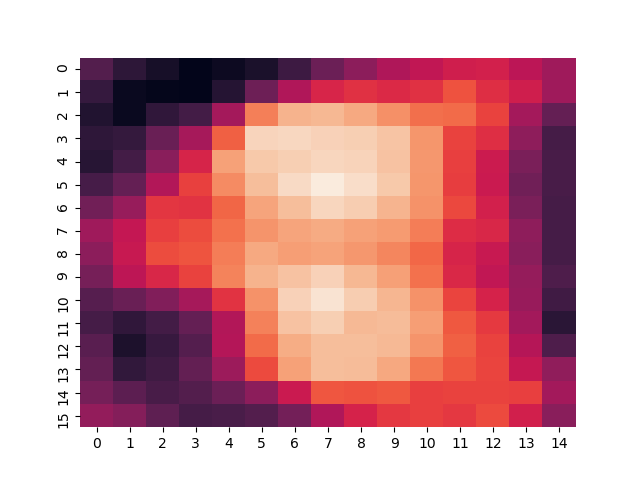
\includegraphics[scale=.07]{img/sample/1}}
    \subfloat[][]{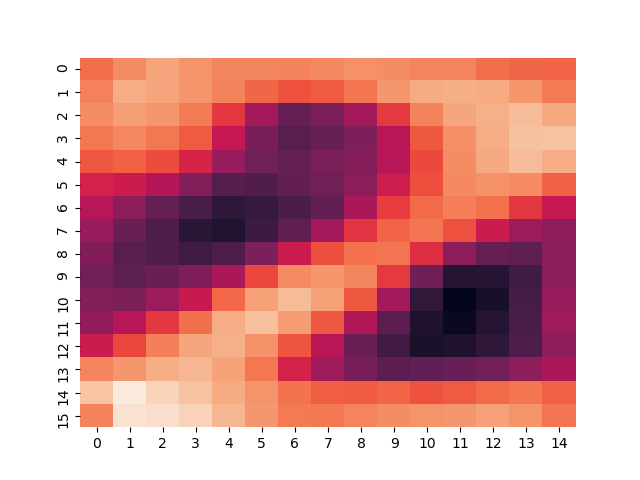
\includegraphics[scale=.07]{img/sample/2}}
    \subfloat[][]{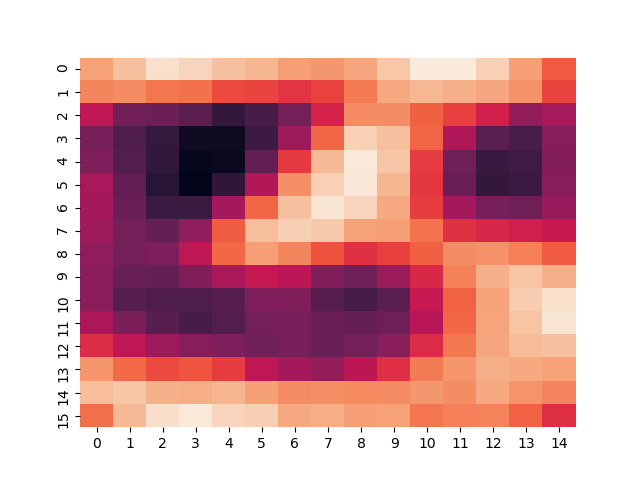
\includegraphics[scale=.07]{img/sample/3}}
    \subfloat[][]{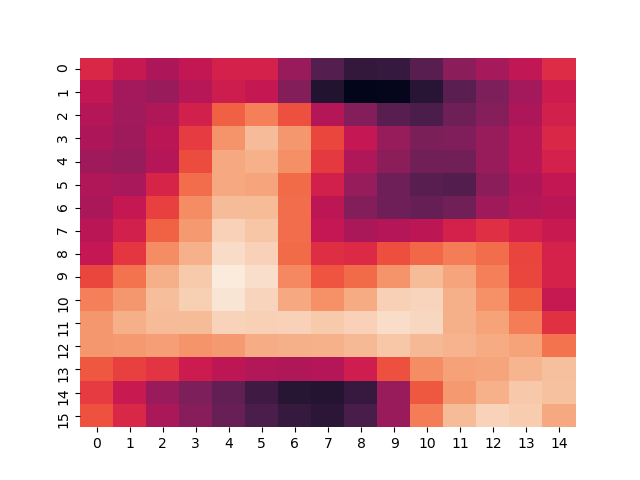
\includegraphics[scale=.07]{img/sample/4}}
    \subfloat[][]{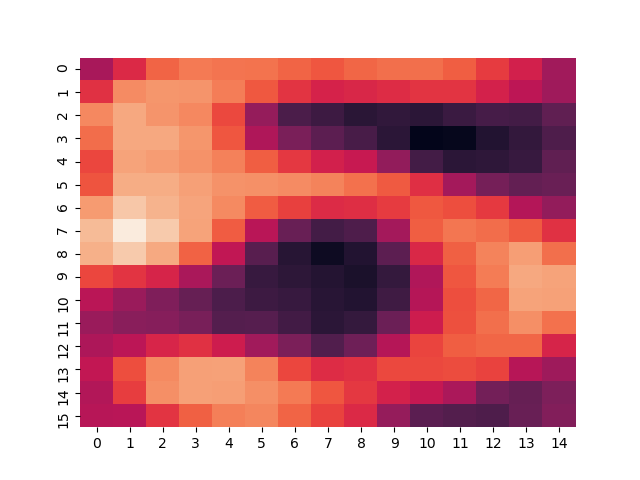
\includegraphics[scale=.07]{img/sample/5}}
    \subfloat[][]{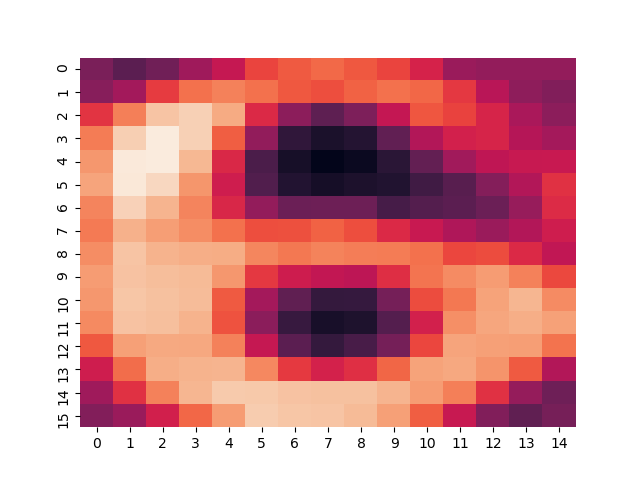
\includegraphics[scale=.07]{img/sample/6}}
    \subfloat[][]{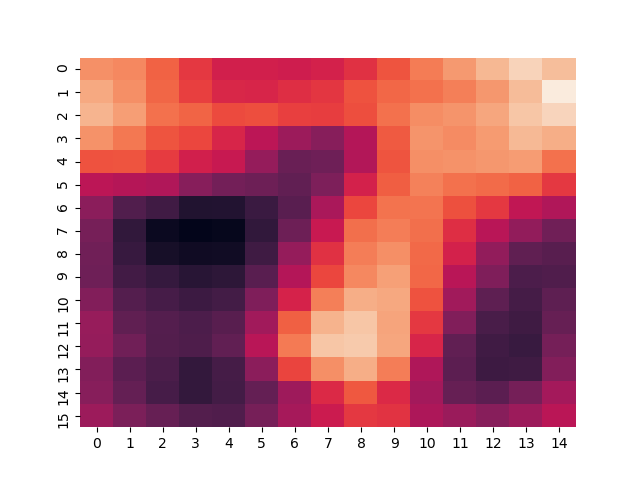
\includegraphics[scale=.07]{img/sample/7}}
    \subfloat[][]{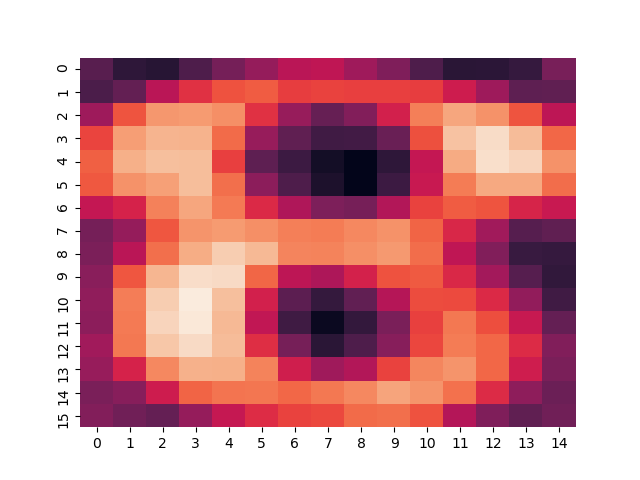
\includegraphics[scale=.07]{img/sample/8}}
    \subfloat[][]{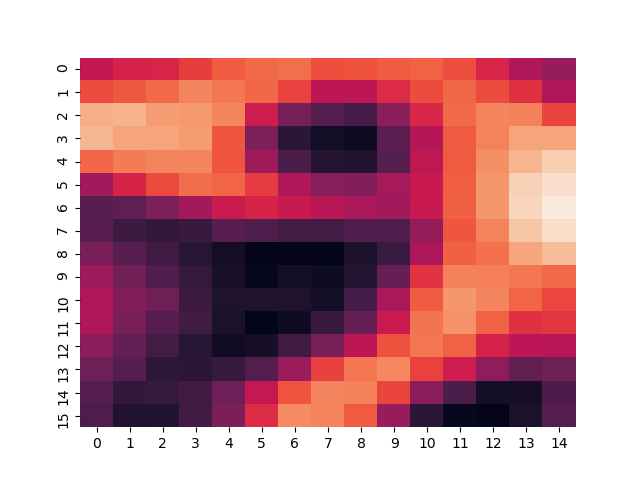
\includegraphics[scale=.07]{img/sample/9}}
    \caption{Échantillon d'images bien reconstruites pour le jeu de données MFDD.}
\label{fig:num_reconstructed}
\end{figure}

\begin{figure}[h]
    \centering
    \subfloat[][]{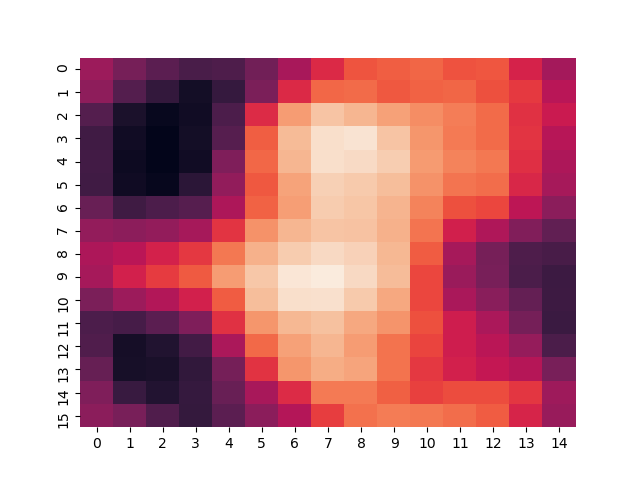
\includegraphics[scale=.07]{img/moches/00}}
    \subfloat[][]{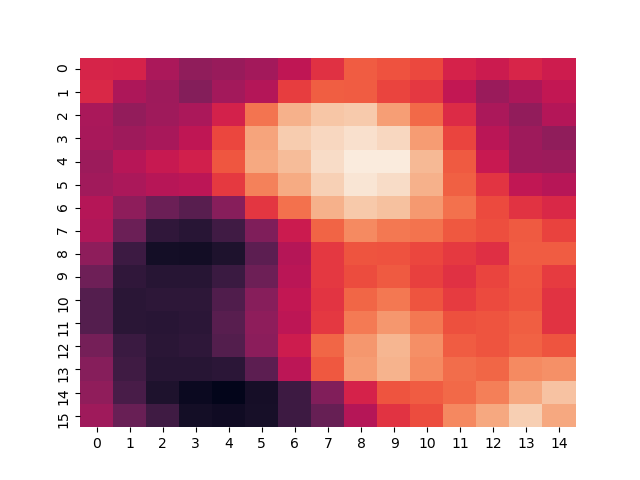
\includegraphics[scale=.07]{img/moches/11}}
    \subfloat[][]{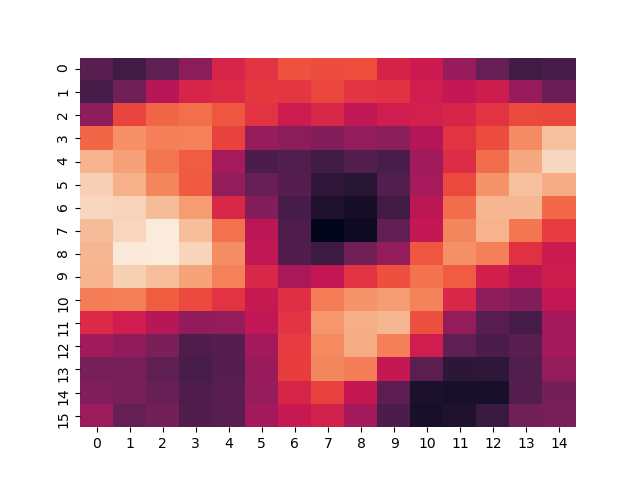
\includegraphics[scale=.07]{img/moches/22}}
    \subfloat[][]{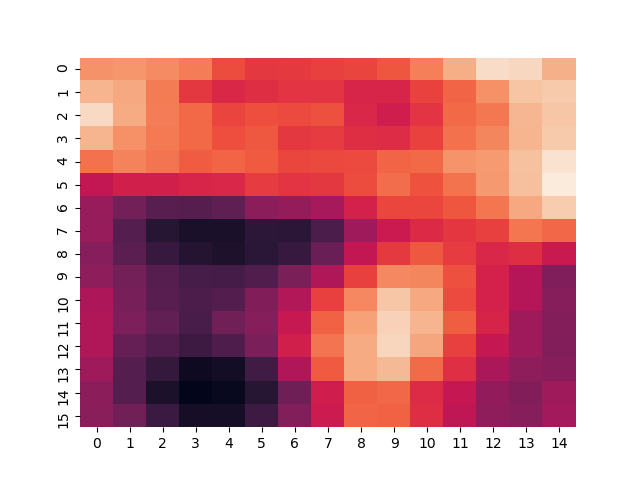
\includegraphics[scale=.07]{img/moches/33}}
    \subfloat[][]{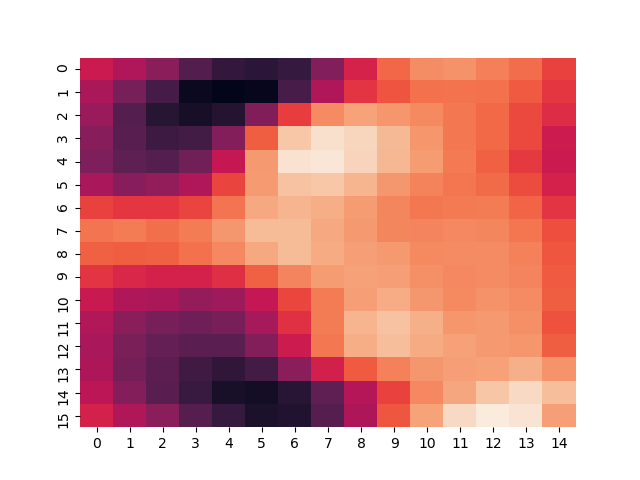
\includegraphics[scale=.07]{img/moches/44}}
    \subfloat[][]{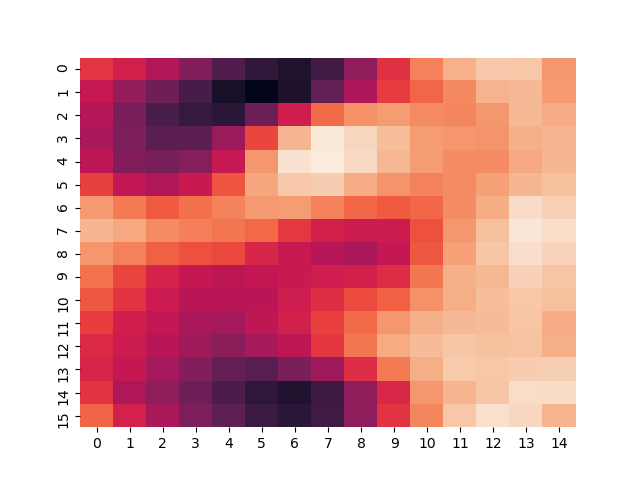
\includegraphics[scale=.07]{img/moches/55}}
    \subfloat[][]{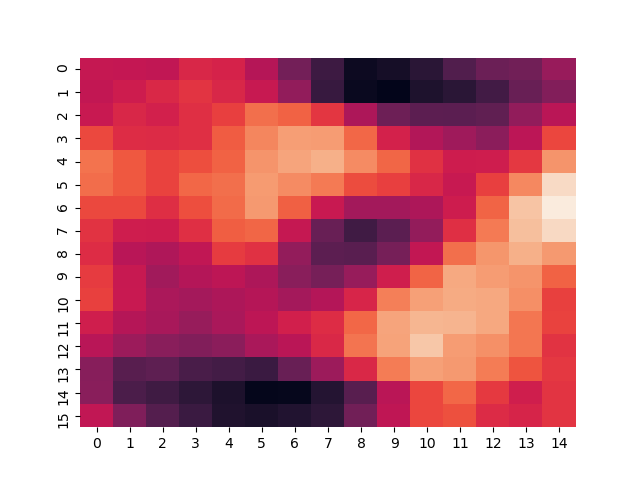
\includegraphics[scale=.07]{img/moches/66}}
    \subfloat[][]{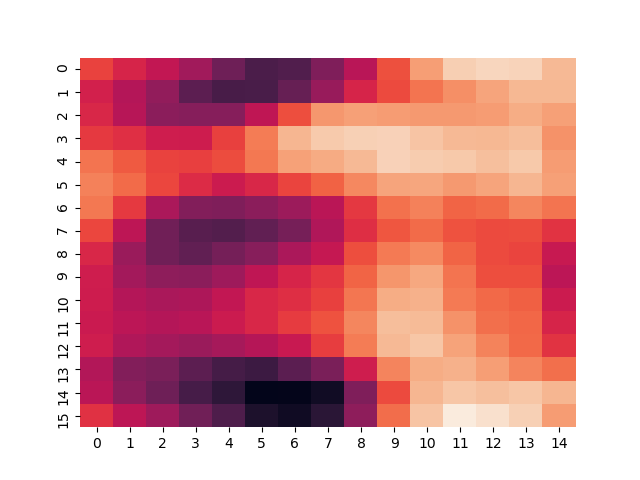
\includegraphics[scale=.07]{img/moches/77}}
    \subfloat[][]{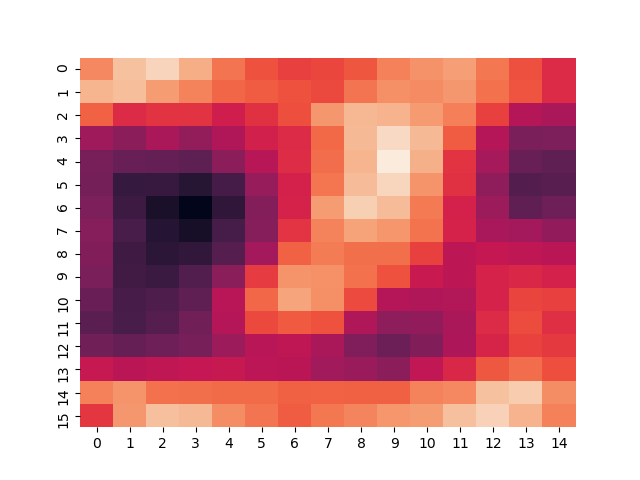
\includegraphics[scale=.07]{img/moches/88}}
    \subfloat[][]{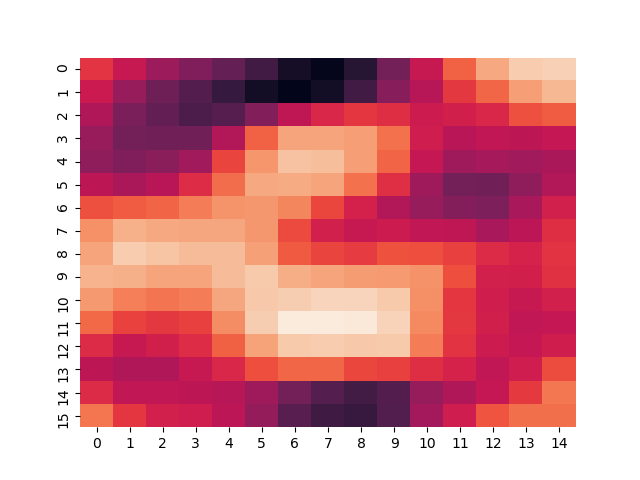
\includegraphics[scale=.07]{img/moches/99}}
    \caption{Échantillon d'images mal reconstruites pour le jeu de données MFDD.}
\label{fig:num_reconstructed_bad}
\end{figure}



Expérimentalement, le système obtient des résultats en terme d'erreur quadratique (relativement à chaque caractéristique) plutôt moyens (Figure~\ref{fig:msemrd}). Cependant on constate sur un échantillon graphique que la reconstruction globale des individus présente une qualité qui permet de reconnaître l'individu initial. C'est aussi ce que montre les résultats en terme de classification présentés sur la Figure~\ref{fig:classif}. Bien que les reconstructions ne soient pas exactement fidèles aux originales, elles sont suffisamment précises pour obtenir des scores en classification proches de ceux obtenus sur les données originales. En résumé, le système arrive à récupérer certaines informations caractéristiques des individus et à les retranscrire, bien que la qualité de la reconstruction en elle même soit améliorable.

\begin{figure}[h]
\label{fig:msemrd}
    \centering
    \subfloat[][WDBC]{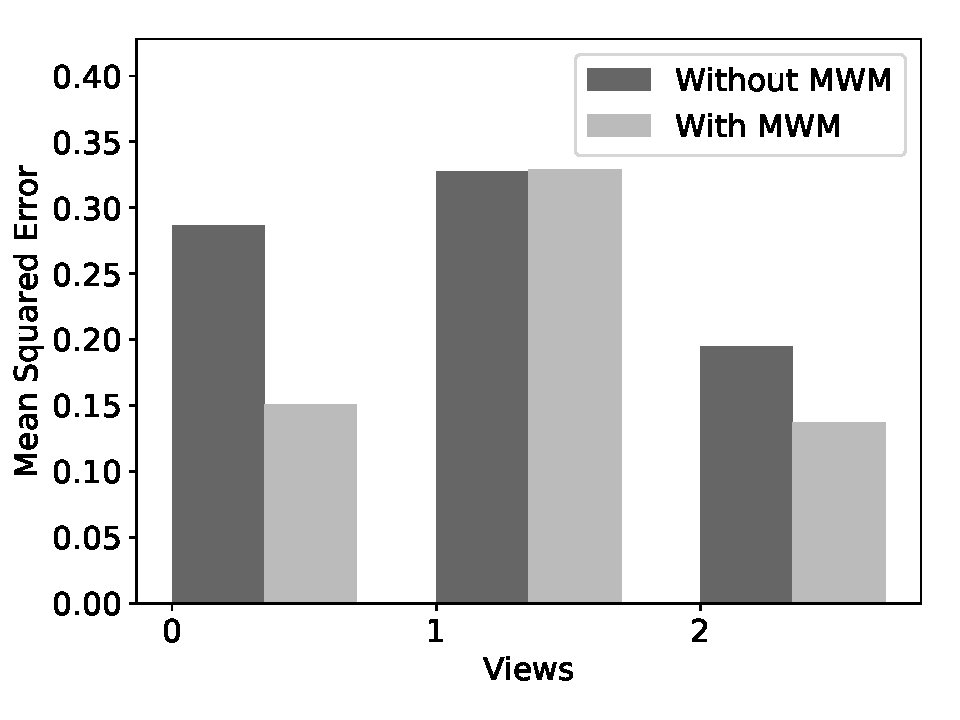
\includegraphics[width=.35\textwidth]{img/mse_wdbc}\label{fig:mse_a}}
    \qquad
    \subfloat[][MFDD]{\includegraphics[width=.35\textwidth]{img/mse_mfeat}\label{fig:mse_b}}\\
    \subfloat[][Madelon]{\includegraphics[width=.35\textwidth]{img/mse_madelon}\label{fig:mse_c}}
    \qquad
    \subfloat[][Cube]{\includegraphics[width=.35\textwidth]{img/mse_cube}\label{fig:mse_d}}
    \caption{Erreur quadratique moyenne pour tous les jeux de données. Une valeur plus faible correspond à un meilleur résultat.}
\end{figure}

\begin{figure}[h]
\label{fig:classif}
    \centering
    \subfloat[][WDBC]{\includegraphics[scale=.30]{img/cd_wdbc}\label{fig:classif_c}}
    \quad
    \subfloat[][MFDD]{\includegraphics[scale=.30]{img/cd_mfeat}\label{fig:classif_d}}\\
    \subfloat[][Madelon]{\includegraphics[scale=.30]{img/cd_madelon}\label{fig:classif_f}}
    \quad
    \subfloat[][Cube]{\includegraphics[scale=.30]{img/cd_cube}\label{fig:classif_h}}
    \caption{Scores et Différences de Classification pour WDBC, MFDD et Madelon. Une valeur au dessus de 0 indique que les classifications effectués à l'aide des données reconstruites sont meilleures que celles basées sur les données originales.}
\end{figure}

Comme présenté sur la Figure~\ref{fig:classif} et~\ref{fig:msemrd}, le test indiquant l'efficacité de la méthode de pondération par masque par rapport à une moyenne indique que notre méthode améliore sensiblement la qualité de reconstruction des individus. De plus, les tests conduits sur Cube montrent clairement que notre méthode arrive à détecter automatiquement quels caractéristiques sont à privilégier suivant la vue externe considérée. En effet, les valeurs des coefficient portant sur la caractéristique que les vues ont en commun avoisine toujours 0.92, tandis que les autres sont proches de 0.14, indiquant un favoritisme fort pour les caractéristiques en commun. Les résultats concernant la classification semblent cependant indiquer que notre méthode n'apporte pas d'amélioration significative de ce point de vue là.

Pour conclure cette section, nous avons défini un nouveau contexte d'apprentissage collaboratif permettant de reconstruire des individus manquant à partir d'informations présentes dans d'autres vues. Une nouvelle méthode de pondération collaborative a été définie et testée. Le système, bien que présentant des résultats améliorables en terme de reconstruction, permet de capturer des informations intrinsèques aux individus telles que leur classe, et la méthode de pondération arrive à identifier clairement quels caractéristiques sont à privilégier lorsque plusieurs sources sont disponibles pour la reconstruction.

\section{Résumé des contributions scientifiques et perspectives}

\subsection{Contributions au clustering collaboratif}

Durant cette thèse, nous avons pu définir une nouvelle méthode permettant d'apprendre automatiquement les coefficient définissant l'importance qu'une vue doit accorder à l'information fournie par une de ses paires. Le fondement théorique de cette méthode se base sur la définition d'un problème d'optimisation sous contrainte que nous avons résolu à l'aide de la méthode de Karush-Kuhn-Tucker.
Notre seconde contribution a consisté en la définition d'une nouvelle méthode permettant d'apprendre des cartes auto adaptatrices au cours du temps. Cette méthode présente l'avantage de ne pas dépendre de modifications topologiques, ce qui a permis son adaptation au clustering collaboratif. Cette méthode se base essentiellement sur la redéfinition de la fonction de châleur à la base des cartes auto adaptatrices pour faire en sorte qu'elle dépende de l'arrivée des nouvelles données plutôt que du temps.

\subsection{Contribution à la reconstruction collaborative}

L'étude des communications au sein des modèles collaboratifs nous a permis de définir un nouveau contexte d'apprentissage permettant de reconstruire des données manquantes localement à l'aide des informations contenues dans les vues externes. Afin de proposer une première approche, nous avons défini un système basé sur les réseaux de neurones et sur une nouvelle méthode de pondération. Nous avons pu tester son efficacité ainsi que l'efficacité de notre méthode de pondération sur des cas variés montrant que le système était capable de capturer et de reconstruire suffisamment d'informations pour permettre l'indentification graphique et le classement des individus reconstruits.

\subsection{Perspectives}

Plusieurs axes de recherches peuvent être développés à court et long terme en se basant sur les travaux eeffectués lors de cette thèse. 

\subsubsection{Perspectives à court termes}

Concernant l'optimisation des pondérations dans un contexte multi-vues, des extensions possibles peuvent s'appliquer au clustering collaboratif vertical pour lequel les cartes auto adaptatrices doivent gérer des informations décrites par un même ensemble de caractéristiques appliquées à un ensemble d'individus différents. De plus, l'application des méthodes décrites dans cette thèse à des algorithmes de clustering tels que les Generative Topographic Maps peut être envisagée dans un premier temps, puis à des méthodes de clustering non topologiques dans un second temps.

Comme présenté dans la section ci-dessus, les résultats obtenus à l'aide du système de reconstruction collaborative sont encore perfectibles du point de vue du détail de reconstruction. Bien que les résultats préliminaires soient encourageant, des recherches approfondies seraient menées à court termes sur le lien entre la taille du code utilisé pour le transfert de données et les difficultées rencontrés par les perceptrons multi-couches lors de leur entraînement. De même, l'application de la méthode de pondération par masques sera étudiée dans des contextes collaboratifs autres que celui de la reconstruction.

\subsubsection{Perspectives à long termes}
À plus long terme, l'étude de l'information transférée d'une vue à une autre et l'utilisation qu'il est possible d'en faire permettra de faire avancer le domaine de l'apprentissage collaboratif. De nos jours, la sécurité des données sont des sujets vivement étudiés qui doivent prendre en considération les différentes utilisations qui sont faites des données, et le contexte collaboratif se prête particulièrement bien à ce genre de réflexions et de recherches. Nos travaux dans le domaine de la reconstruction se basent sur des Auto-encodeurs pour fournir un minimum de sécurité, mais cette solution n'est pas satisfaisante sur le long terme.

Enfin, l'étude théorique d'un framework collaboratif permettant son application à des cas d'utilisations autre que la reconstruction et le clustering pourrait s'avérer utile. L'échange d'informations entre deux vues liées à la fois par des intérêts (obtenir de nouvelles informations pour améliorer les résultats locaux) et par des contraintes (partage de données sensibles) est un concept qui sera utilisé comme base pour de futures recherches.


    \bibliographystyle{plain}
    \bibliography{bib.bib}
\end{document}
